\documentclass{article}
%\usepackage[english]{babel}%
\usepackage{graphicx}
%\usepackage{tabu}
\usepackage{makecell}
\usepackage{tabularx}
\usepackage{tabulary}
\usepackage{array}% http://ctan.org/pkg/array
\usepackage{pbox}
\usepackage{multirow}
\usepackage[table]{xcolor}
\usepackage{lastpage}
\usepackage{fixltx2e}
\usepackage[T1]{fontenc}
\usepackage[utf8]{inputenc}
\usepackage{ifthen}
\usepackage{fancyhdr}
\usepackage[document]{ragged2e}
\usepackage[margin=1in,top=1.2in,headheight=57pt,headsep=0.1in, landscape]
{geometry}
\usepackage{ifthen}
\usepackage{fancyhdr}
\usepackage{enumitem}
\usepackage{pdflscape}
\usepackage{float}
\newcolumntype{C}[1]{>{\centering\arraybackslash}m{#1}}

\everymath{\displaystyle}
\linespread{2}%controls the spacing between lines. Bigger fractions means crowded lines%
%\pagestyle{fancy}
%\usepackage[margin=1 in, top=1in, includefoot]{geometry}
%\everymath{\displaystyle}
\linespread{2}%controls the spacing between lines. Bigger fractions means crowded lines%
%\pagestyle{fancy}
\pagestyle{fancy}
\setlength{\headheight}{56.2pt}
\chead{\ifthenelse{\value{page}=1}{
\includegraphics[scale=0.3]{SCC}\\}}
\rhead{\ifthenelse{\value{page}=1}{Shabbir Basrai}{Shabbir Basrai}}
\lhead{\ifthenelse{\value{page}=1}{\textbf Tables}}
\cfoot{}
\cfoot{\thepage\ of \pageref{LastPage}}
\renewcommand{\headrulewidth}{2pt}
\renewcommand{\footrulewidth}{1pt}


\begin{document}

\begin{center}
     \begin{tabular}{ | C{2cm} | C{2cm} | C{2cm} | m{5cm} |}
     \hline
     Day & Min Temp & Max Temp & Summary \\ \hline
     Monday & 11C & 22C & A clear day with lots of sunshine. 
     However, the strong breeze will bring down the temperatures. \\ \hline
     Tuesday & 9C & 19C & Cloudy with rain, across many northern regions. Clear spells
     across most of Scotland and Northern Ireland,
     but rain reaching the far northwest. \\ \hline
     Wednesday & 10C & 21C & Rain will still linger for the morning.
     Conditions will improve by early afternoon and continue
     throughout the evening. \\
     \hline
     \end{tabular}
\end{center}


\renewcommand{\arraystretch}{0.6}
\begin{tabular}{ | m {4 cm} | m {4 cm}| m{4 cm} |} 
 \hline
Raw sludge pumping schedule & 12 min/hr & \\ 
 \hline
Sludge pumping rate & 68 GPM &\\ 
 \hline
 Raw sludge \%TS & 5.2\% & \\
 \hline
  Raw sludge \%VS & 72.5\% &  \\
 \hline
 Digester sludge \%VS & 56\% & \\
 \hline
Gas production & $\frac{12 ft^3}{lb \enspace VS \enspace destroyed \enspace - \enspace day}$ & \\
 \hline
 Percent $CO_2$ & 34\% &\\ 
 \hline
 Other gases & 1\% & \\
 \hline
  Pure methane net heat value & 932 $\frac{BTU}{ft^3}$ & \\
 \hline
\end{tabular}\\

\begin{tabular}{ | m {7 cm} | m {7 cm}| } 
 \hline
Two aeration tanks – 0.5 MG each & Two final clarifiers – 0.25 MG each \\ 
 \hline
 Final effluent $= 20\frac{mg}{l}$ & WAS = 7500 ppm\\ 
 \hline
 MLSS =$3600\frac{mg}{L}$ & MLSS volatile solids content = 80\%  \\
 \hline
\end{tabular}\vspace{5 cm}
\\ 
\begin{tabular}{ |p{3cm}||p{3cm}|p{3cm}|p{3cm}|  }
 \hline
 \multicolumn{4}{|c|}{Country List} \\
 \hline
 Country Name     or Area Name& ISO ALPHA 2 Code &ISO ALPHA 3 Code&ISO numeric Code\\
 \hline
 Afghanistan   & AF    &AFG&   004\\
 Aland Islands&   AX  & ALA   &248\\
 Albania &AL & ALB&  008\\
 Algeria    &DZ & DZA&  012\\
 American Samoa&   AS  & ASM&016\\
 Andorra& AD  & AND   &020\\
 Angola& AO  & AGO&024\\
 \hline
\end{tabular}\\
%_________________________________________________________________
\vspace{2cm}
%\begin{tabu} to 1\textwidth { | X[l] | X[c] | X[r] | }
% \hline
% item 11 & item 12 & item 13 \\
% \hline
% item 21  & item 22  & item 23  \\
%\hline
%\end{tabu}
%
%\begin{center}
%%\usepackage{multirow}
%\begin{tabular}{ |c|c|c|c| } 
%\hline
%col1 & col2 & col3 \\
%\hline
%\multirow{3}{5cm}{Multiple row 1} & cell2 & cell3 \\ 
%& cell5 & cell6 \\ 
%& cell8 & cell9 \\
%\hline
%\multirow{3}{5cm}{Multiple row 2} & cell2 & cell3 \\ 
%& cell5 & cell6 \\ 
%& cell8 & cell9 \\
%\hline
%\end{tabular}
%\end{center}
%_______________________________________________

{\rowcolors{3}{green!80!yellow!50}{green!70!yellow!40}
\begin{tabular}{ |p{3cm}|p{3cm}|p{3cm}|  }
\hline
\multicolumn{3}{|c|}{Country List} \\
\hline
Country Name     or Area Name& ISO ALPHA 2 Code &ISO ALPHA 3 \\
\hline
Afghanistan & AF &AFG \\
Aland Islands & AX   & ALA \\
Albania &AL & ALB \\
Algeria    &DZ & DZA \\
American Samoa & AS & ASM \\
Andorra & AD & AND   \\
Angola & AO & AGO \\
\hline
\end{tabular}
}
%_______________________________________________

\setlength{\arrayrulewidth}{1mm}
\setlength{\tabcolsep}{18pt}
\renewcommand{\arraystretch}{2.5}

{\rowcolors{3}{green!80!yellow!50}{green!70!yellow!40}
\begin{tabular}{ |p{3cm}|p{3cm}|p{3cm}|  }
\hline
\multicolumn{3}{|c|}{Country List} \\
\hline
Country Name     or Area Name& ISO ALPHA 2 Code &ISO ALPHA 3 \\
\hline
Afghanistan & AF &AFG \\
Aland Islands & AX   & ALA \\
Albania &AL & ALB \\
Algeria    &DZ & DZA \\
American Samoa & AS & ASM \\
Andorra & AD & AND   \\
Angola & AO & AGO \\
\hline
\end{tabular}
}
%_______________________________________________
\setlength{\arrayrulewidth}{1mm}
\setlength{\tabcolsep}{18pt}
\renewcommand{\arraystretch}{2.5}
 
\newcolumntype{s}{>{\columncolor[HTML]{AAACED}} p{3cm}}
 
\arrayrulecolor[HTML]{DB5800}
 
\begin{tabular}{ |s|p{3cm}|p{3cm}|  }
\hline
\rowcolor{lightgray} \multicolumn{3}{|c|}{Country List} \\
\hline
Country Name    or Area Name& ISO ALPHA 2 Code &ISO ALPHA 3 \\
\hline
Afghanistan & AF &AFG \\
\rowcolor{gray}
Aland Islands & AX & ALA \\
Albania   &AL & ALB \\
Algeria  &DZ & DZA \\
American Samoa & AS & ASM \\
Andorra & AD & \cellcolor[HTML]{AA0044} AND    \\
Angola & AO & AGO \\
\hline
\end{tabular}

%_______________________________________________
\setlength{\arrayrulewidth}{1mm}
\setlength{\tabcolsep}{18pt}
\renewcommand{\arraystretch}{2.5}

{\rowcolors{3}{green!80!yellow!50}{green!70!yellow!40}
\begin{tabular}{ |p{3cm}|p{3cm}|p{3cm}|  }
\hline
\multicolumn{2}{|c|}{Country List} & \\
\hline
Country Name     or Area Name& ISO ALPHA 2 Code &ISO ALPHA 3 \\
\hline
Afghanistan & AF &AFG \\
Aland Islands & AX   & ALA \\
Albania &AL & ALB \\
Algeria    &DZ & DZA \\
American Samoa & AS & ASM \\
Andorra & AD & AND   \\
Angola & AO & AGO \\
\hline
\end{tabular}
}
%_______________________________________________
\setlength{\arrayrulewidth}{1mm}
\setlength{\tabcolsep}{18pt}
\renewcommand{\arraystretch}{2.5}
 
\newcolumntype{s}{>{\columncolor[HTML]{AAACED}} p{3cm}}
 
\arrayrulecolor[HTML]{DB5800}
 
\begin{tabular}{ |s|p{3cm}|p{3cm}|  }
\hline
\rowcolor{lightgray} \multicolumn{3}{|c|}{Country List} \\
\hline
Country Name    or Area Name& ISO ALPHA 2 Code &ISO ALPHA 3 \\
\hline
Afghanistan & AF &AFG \\
\rowcolor{gray}
Aland Islands & AX & ALA \\
Albania   &AL & ALB \\
Algeria  &DZ & DZA \\
American Samoa & AS & ASM \\
Andorra & AD & \cellcolor[HTML]{AA0044} AND    \\
Angola & AO & AGO \\
\hline
\end{tabular}\\
%_______________________________________________
\begin{tabular}{  m {7 cm}  m {7 cm} } 
\begin{center} 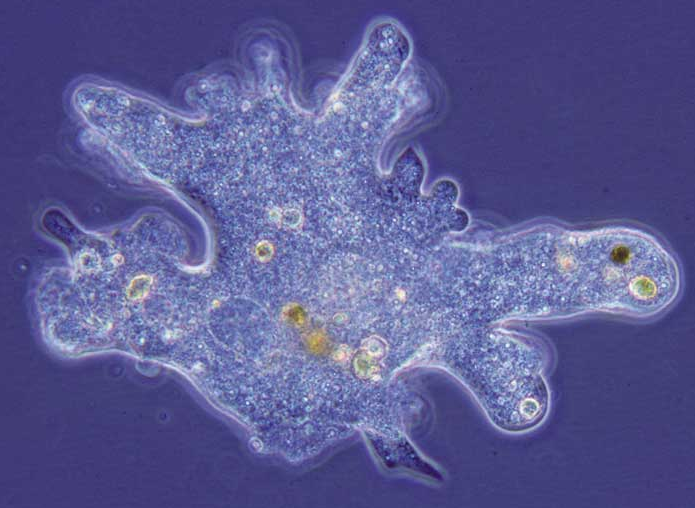
\includegraphics[scale=0.35]{Amoeba} \end{center} & \begin{center}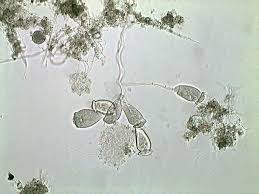
\includegraphics[scale=0.88]{StalkedCilliate} \end{center}\\
\begin{center} \textbf{Amoeba} \end{center} & \begin{center}\textbf{StalkedCilliate} \end{center}\\
\begin{center} 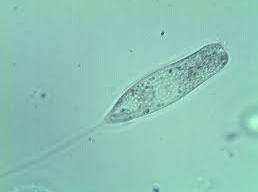
\includegraphics[scale=0.88]{Flagellate} \end{center} & \begin{center}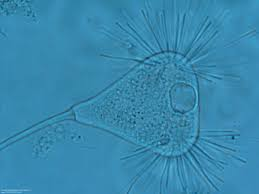
\includegraphics[scale=0.88]{Suctorian} \end{center}\\
\begin{center} \textbf{Flagellate} \end{center} & \begin{center}\textbf{Suctorian} \end{center}\\
\end{tabular}\\
%________________________________________________
%This uses \usepackage{makecell}
\renewcommand\theadalign{cb}
\renewcommand\theadfont{\bfseries}
\renewcommand\theadgape{\Gape[4pt]}
\renewcommand\cellgape{\Gape[4pt]}


\begin{center}
\begin{tabular}{ | c | c | c |}
\hline
\thead{A Head} & \thead{A Second \\ Head} & \thead{A Third \\ Head} \\
\hline
Some text &  \makecell{Some really \\ longer text}  & Text text text  \\
\hline
\end{tabular}
\end{center}

%this uses \usepackage{pbox}

\begin{tabular}{|l|l|} \hline
    \pbox{20cm}{This is the first \\ cell} & second \\ \hline
    3rd & and the last cell \\ \hline
\end{tabular}\\

\setlength{\arrayrulewidth}{1mm}
\setlength{\tabcolsep}{8 pt}
\renewcommand{\arraystretch}{0.7}

{\rowcolors{3}{blue!80!yellow!50}{green!70!yellow!40}
\begin{tabular}{ |p{4cm}|p{4.5cm}|p{6.5cm}|  }
\hline
\multicolumn{3}{|c|}{\textbf{Wastewater Chemicals}} \\
\hline
%\thead{A Head} & \thead{A Second \\ Head} & \thead{A Third \\ Head} \\
%\hline%

\hspace{1 cm}PROCESS & \hspace{0.8 cm} ACTION & \hspace{1.2 cm} CHEMICAL USED \\
\hline
Collections & Odor Control & Caustic Soda (pH control) \newline Magnesium Hydroxide (pH control) \newline Hydrogen Peroxide (Oxidant) \newline Sodium Nitrate (Bio. Degradation)\newline Iron Salts (Precipitant)\\
Primary & CEPT & Ferric Chloride (Coagulant) \newline Anionic Polymer (Flocculant) \\
Secondary    &Filament Control & Bleach \newline Polymer \\
Nutrient Removal & Phosphorous Removal & Iron Salts (Precipitant) \\
Anaerobic Digestion & pH control & \\
Tertiary Treatment & Disinfection  \newline Dechlorination & Chlorine/Bleach \newline Sodium Bisulfite  \newline Sulfur Dioxide   \\
Dewatering & Flocculation & Cationic Polymer \\
Plant Odor Control & Foul Air Scrubbing & Hydrogen Peroxide (Oxidant) \newline Bleach (Oxidant) \newline Caustic Soda (pH Control) \newline Muriatic Acid (pH Control \& Scrubber Descaling)\\
\hline
Anaerobic Digestion & Hydrogen Sulfide Control & Iron Salts (Precipitant) \\
\hline
\end{tabular}
}\\
\begin{tabular}{llr}
\hline
\multicolumn{2}{c}{Item} \\
\cline{1-2}
Animal    & Description & Price (\$) \\
\hline
Gnat      & per gram    & 13.65      \\
          & each        & 0.01       \\
Gnu       & stuffed     & 92.50      \\
Emu       & stuffed     & 33.33      \\
Armadillo & frozen      & 8.99       \\
\hline
\end{tabular}

\begin{table}[h!]
  \centering
  \begin{tabular}{ | c | m{5cm} | m{5cm} | }
    \hline
    my.Lboro & Advantages & Disadvantages \\ \hline
    \begin{minipage}{.3\textwidth}
      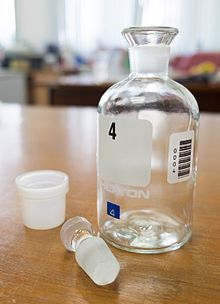
\includegraphics[width=\linewidth, height=60mm]{LaboratoryBODBottlePicture}
    \end{minipage}
    &
    %\begin{minipage}[t]{5cm}
      \begin{itemize}
        \item Accessibility
        \item Up to date information
        \item Fulfil students needs and wants \ldots
      \end{itemize}
    %\end{minipage}
    & 
    %\begin{minipage}{5cm}
      \begin{itemize}
        \item Accessibility
        \item Up to date information
        \item Fulfil students needs and wants \ldots
      \end{itemize}
    %\end{minipage}
    \\ \hline
  \end{tabular}
  \caption{my.Lboro Analysis}\label{tbl:myLboro}
\end{table}

\begin{center}
    \begin{tabular}{ | l | l | l | p{5cm} |}
    \hline
    Day & Min Temp & Max Temp & Summary \\ \hline
    Monday & 11C & 22C & A clear day with lots of sunshine.  
    However, the strong breeze will bring down the temperatures. \\ \hline
    Tuesday & 9C & 19C & Cloudy with rain, across many northern regions. Clear spells 
    across most of Scotland and Northern Ireland, 
    but rain reaching the far northwest. \\ \hline
    Wednesday & 10C & 21C & Rain will still linger for the morning. 
    Conditions will improve by early afternoon and continue 
    throughout the evening. \\
    \hline
    \end{tabular}
\end{center}
\pagebreak
You may also specify the skip after a line explicitly using glue after the line terminator\\
\begin{tabular}{ll}
\hline
Mineral & Color \\[1cm]
Ruby & red \\
Sapphire & blue \\
\hline
\end{tabular}

\setlength{\tabcolsep}{5pt}
\renewcommand{\arraystretch}{1.5}
\begin{tabular}{ll}
\hline
Mineral & Color \\[1cm]
Ruby & red \\
Sapphire & blue \\
\hline
\end{tabular}


\setlength{\tabcolsep}{100pt}
\renewcommand{\arraystretch}{1.5}
\begin{tabular}{ll}
\hline
Mineral & Color \\[1cm]
Ruby & red \\
Sapphire & blue \\
\hline
\end{tabular}\\
\pagebreak
An alternative way to adjust the rule spacing is to add %\noalign{\smallskip} before or after the \hline and \cline{i-j} commands:

\begin{tabular}{ | l | l | r | }
  \hline\noalign{\smallskip}
  \multicolumn{2}{c}{Item} \\
  \cline{1-2}\noalign{\smallskip}
  Animal & Description & Price (\$) \\
  \noalign{\smallskip}\hline\noalign{\smallskip}
  Gnat  & per gram & 13.65 \\
        & each     &  0.01 \\
  Gnu   & stuffed  & 92.50 \\
  Emu   & stuffed  & 33.33 \\
  Armadillo & frozen & 8.99 \\
  \noalign{\smallskip}\hline
\end{tabular}

\begin{tabular}{|c||c|c|} \hline
%%%%%% Title row starts here
& A & B \\ \hline\hline
%%%%%% Row Foo starts here
Foo &
\begin{tabular}{c} 1 \\ 2 \\ 3 \\ 4 \\
\end{tabular} &
\begin{tabular}{c} 2 \\ 5 \\ 9 \\ 8 \\
\end{tabular} \\ \hline
%%%%%% Row Bar starts here
Bar &
\begin{tabular}{c} 1 \\ 2 \\ 3 \\ 4 \\
\end{tabular} &
\begin{tabular}{c} 31 \\ 23 \\ 16 \\ 42 \\
\end{tabular} \\ \hline
\end{tabular}


\begin{tabular}{c c c c}
\textbf{Time} & \textbf{Flow, MGD} & \textbf{Time} & \textbf{Flow, MGD}\\
06:00 AM & 5.8 & 12:00 pm & 9.0\\
07:00 AM & 6.4 & 01:00 pm & 9.6\\
08:00 AM & 6.8 & 02:00 pm & 8.8\\
09:00 AM & 7.2 & 03:00 pm & 8.2\\
10:00 AM & 6.8 & 04:00 pm & 7.6\\
11:00 AM & 7.2 & 05:00 pm & 6.8\\
\end{tabular}\\

\newpage
\newgeometry{top=20mm, bottom=10mm} 
\pagestyle{empty}
\begin{center}
\textbf{Types of Distribution Systems}
\end{center}
\vspace{-2em}


\begin{table}[h!]
  \centering
  \begin{tabular}{  c m{4cm} | m{3.1cm} |  m{3.1cm} |}
    \hline
\multicolumn{2}{c}{Dead-end or Tree Distribution System} & Advantages & Disadvantages\\ \hline
    \begin{minipage}{.3\textwidth}
%    \tcbox[colframe=green!30!black,
%           colback=green!30]{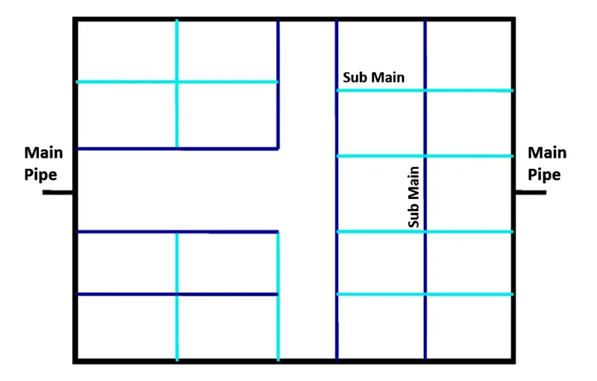
\includegraphics[scale=0.5]{RingDistributionSystem}}    
     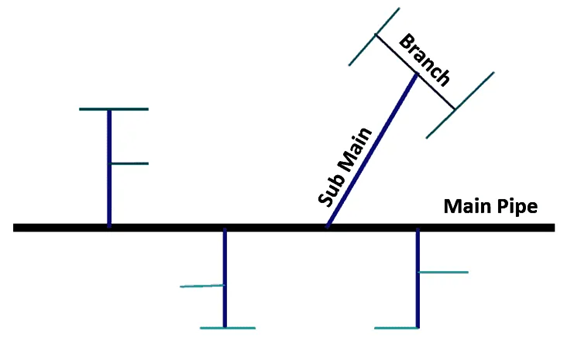
\includegraphics[scale=0.25]{DeadEndTreeDistributionSystem}\\
    \end{minipage}
    &
  \scriptsize{In this type of water distribution system, one main pipeline runs through the center of the building, and the sub-mains branch lines off from both sides. The sub-main lines are  divided into several branch lines for service connection to a particular house.}  
  \vspace{-2em} 
    &
    \vspace{0.2cm}
    %\begin{minipage}[t]{5cm}
      \begin{itemize}[leftmargin=*]
      \scriptsize{
        \item Pipe laying is simple and easy.
        \item Fewer cut-off valves are required - lower O\&M costs.
        \item Maintenance done without disrupting flow
        \item Minimal stagnation}
      \end{itemize}
    %\end{minipage}
    & 
    %\begin{minipage}{5cm}
    \vspace{0.2cm}
       \begin{itemize}[leftmargin=*]
      \scriptsize{
        \item Does not maintain satisfactory pressure in high-rise buildings.
        \item As one pipe provides the water to the entire building  - quite risky.
        \item High head loss, req. larger dia. piping
        \item System discharge capacity is limited.}
      \end{itemize}
    %\end{minipage}
    \\ \hline
   \end{tabular}
\end{table}


\vspace{-2em} 


\begin{table}[h!]
  \centering
  \begin{tabular}{  c m{4cm} | m{3.1cm} |  m{3.1cm} |}
    \hline
\multicolumn{2}{c}{Ring Distribution System} & Advantages & Disadvantages\\ \hline
    \begin{minipage}{.3\textwidth}
%    \tcbox[colframe=green!30!black,
%           colback=green!30]{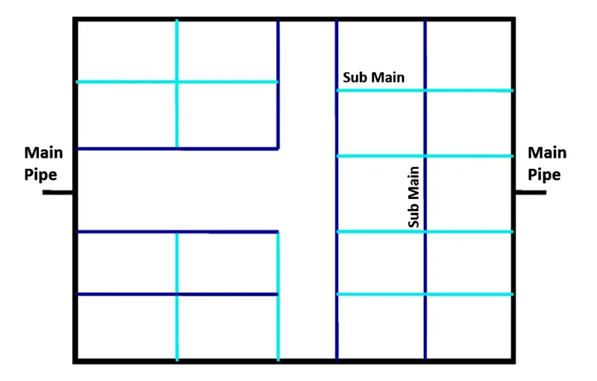
\includegraphics[scale=0.5]{RingDistributionSystem}}    
    \vspace{0.4cm}
     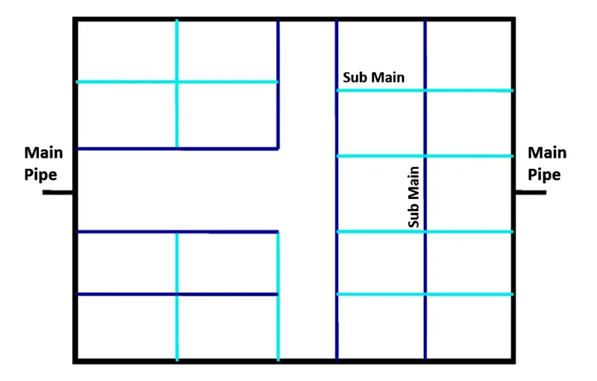
\includegraphics[scale=0.27]{RingDistributionSystem}\\
    \end{minipage}
    &
  \scriptsize{Here, the main pipeline encloses the system.  The branch pipes are connected cross-wise to the mains and also to each other.}  
    &
    %\begin{minipage}[t]{5cm}
        \vspace{0.4cm}
      \begin{itemize}[leftmargin=*]
      \scriptsize{
        \item Discharge rate is high, low head losses
        \item Maintenance can be done without disrupting flow
        \item No endpoints, minimal stagnation}
      \end{itemize}
    %\end{minipage}
    & 
    %\begin{minipage}{5cm}
       \begin{itemize}[leftmargin=*]
      \scriptsize{
        \item The length of pipe laying is more which ultimately leads to higher cost.
        \item Several valves are required to control the flow and discharge of water.}
      \end{itemize}
    %\end{minipage}
    \\ \hline
   \end{tabular}
\end{table}

\vspace{-2em} 
\begin{table}[h!]
  \centering
  \begin{tabular}{  c m{4cm} | m{3.1cm} |  m{3.1cm} |}
    \hline
   \multicolumn{2}{c}{Radial Distribution System} & Advantages & Disadvantages \\ \hline
    \begin{minipage}{.3\textwidth}
%    \tcbox[colframe=green!30!black,
%           colback=green!30]{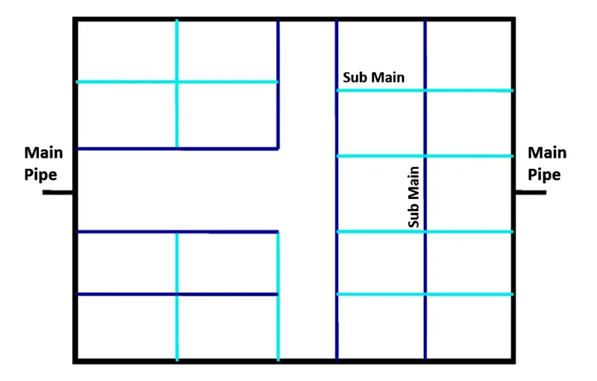
\includegraphics[scale=0.5]{RingDistributionSystem}}    

    \vspace{0.4cm}
    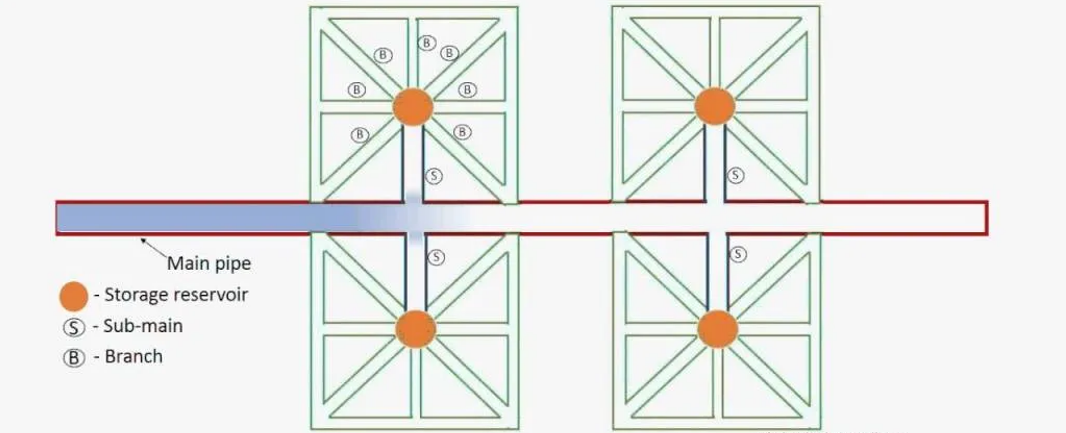
\includegraphics[scale=0.15]{RadialDistributionSystem}\\
    \end{minipage}
    &
  \scriptsize{In this types of water distribution system, the whole buildings are divided into several distribution areas. Each building has a centrally located elevated reservoir from where distribution pipes run radially towards the periphery of the distribution areas.}  
    &
    %\begin{minipage}[t]{5cm}
    \vspace{0.2cm}
      \begin{itemize}[leftmargin=*]
      \scriptsize{
        \item Typically used in high-rise buildings.
        \item Discharge rate is high, low head losses.
        \item Maintenance can be done with minimal flow disruption.
        \item No endpoints, minimal stagnation}
      \end{itemize}
    %\end{minipage}
    & 
    %\begin{minipage}{5cm}
       \begin{itemize}[leftmargin=*]
      \scriptsize{
        \item The design of the pipe laying system is complicated.
        \item More length of pipe is required.}
      \end{itemize}
    %\end{minipage}
    \\ \hline
   \end{tabular}
\end{table}

\vspace{-2em} 


\begin{table}[h!]
  \centering
  \begin{tabular}{  c m{4cm} | m{3.1cm} |  m{3.1cm} |}
    \hline
\multicolumn{2}{c}{Grid Iron Distribution System} & Advantages & Disadvantages\\ \hline
    \begin{minipage}{.3\textwidth}
%    \tcbox[colframe=green!30!black,
%           colback=green!30]{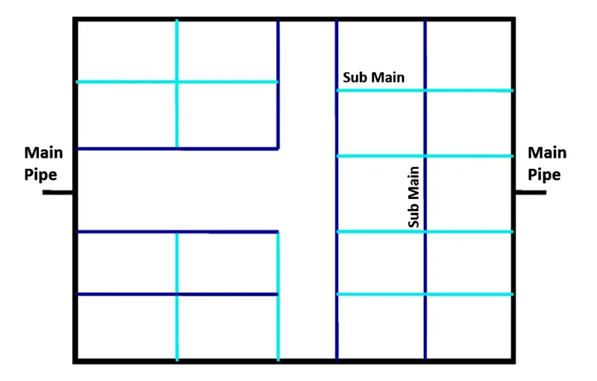
\includegraphics[scale=0.5]{RingDistributionSystem}}    
%   \vspace{0.2cm}
     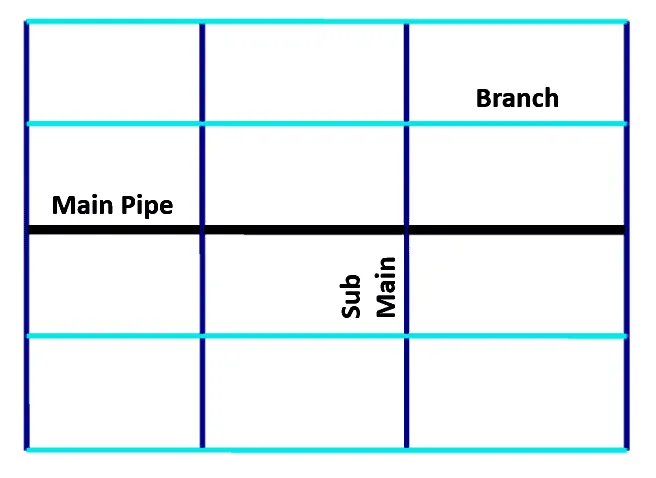
\includegraphics[scale=0.27]{GridIronDistributionSystem}\\
    \end{minipage}
    &
  \scriptsize{Main supply lines run through the center, and sub mains branch off in perpendicular directions. The branch interconnects the sub-mains. All types of pipes are interconnected - no dead ends. Water can reach any given point from many directions, which allows more flexible operation, particularly when repairs are required.}  
    &
    %\begin{minipage}[t]{5cm}
        \vspace{0.2cm}
      \begin{itemize}[leftmargin=*]
      \scriptsize{
        \item Minimal stagnation or sediment deposit.
        \item Water is available at every point with minimum loss of head.
        \item Water is delivered with adequate pressure for firefighting.
        \item During repair, few houses are affected.}
      \end{itemize}
      \vspace{-1em} 
    %\end{minipage}
    & 
    %\begin{minipage}{5cm}
       \begin{itemize}[leftmargin=*]
      \scriptsize{
        \item In this system, more cut-off valves are required.
        \item This system requires longer pipe lengths with larger diameters.
        \item The analysis of discharge, pressure, and velocity in the pipes is difficult and cumbersome.}
      \end{itemize}
    %\end{minipage}
    \\ \hline
   \end{tabular}
\end{table}
\vspace{-2em} 
\restoregeometry

\begin{table}[H]
  \begin{tabular}{ | c m{4cm} | m{3.1cm} |  m{3.1cm} |}
    \hline

\multicolumn{2}{c}{\scriptsize{\textbf{SYSTEM}}} & \scriptsize{ADVANTAGES} & \scriptsize{DISADVANTAGES}\\ \hline

    \begin{minipage}{.3\textwidth}
    \scriptsize{\textbf{Dead-end or Tree Distribution System}}\\
     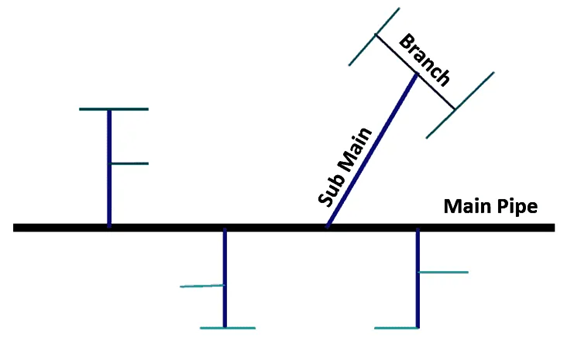
\includegraphics[scale=0.25]{DeadEndTreeDistributionSystem}\\
    \end{minipage}
    &
  \scriptsize{In this type of water distribution system, one main pipeline runs through the center of the building, and the sub-mains branch lines off from both sides. The sub-main lines are  divided into several branch lines for service connection to a particular house.}  
  \vspace{-2em} 
    &
    \vspace{0.2cm}
      \begin{itemize}[leftmargin=*]
      \scriptsize{
        \item Pipe laying is simple and easy.
        \item Fewer cut-off valves are required - lower O\&M costs.
        \item Maintenance done without disrupting flow
        }
      \end{itemize}
    %\end{minipage}
    & 
    %\begin{minipage}{5cm}
    \vspace{0.2cm}
       \begin{itemize}[leftmargin=*]
      \scriptsize{
        \item Does not maintain satisfactory pressure in high-rise buildings.
        \item As one pipe provides the water to the entire building  - quite risky.
        \item High head loss, req. larger dia. piping
        \item System discharge capacity is limited.
        \item Dead-ends can cuase water quality problems and require frequent flushing.}
      \end{itemize}
    %\end{minipage}
    \\ \hline
%\multicolumn{2}{c}{\scriptsize{Ring Distribution System}} & \scriptsize{Advantages} & \scriptsize{Disadvantages}\\ \hline
    \begin{minipage}{.3\textwidth}
    \scriptsize{\textbf{Ring Distribution System}}\\
     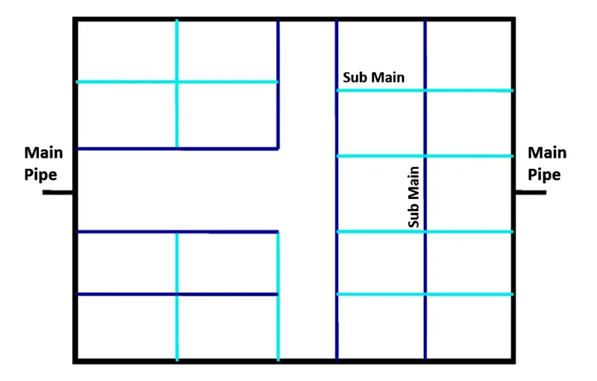
\includegraphics[scale=0.24]{RingDistributionSystem}\\
    \end{minipage}
    &
  \scriptsize{Here, the main pipeline encloses the system.  The branch pipes are connected cross-wise to the mains and also to each other.}  
    &
        \vspace{0.4cm}
      \begin{itemize}[leftmargin=*]
      \scriptsize{
        \item Discharge rate is high, low head losses
        \item Maintenance can be done without disrupting flow
        \item No endpoints, minimal stagnation}
      \end{itemize}
     & 
       \begin{itemize}[leftmargin=*]
      \scriptsize{
        \item The length of pipe laying is more which ultimately leads to higher cost.
        \item Several valves are required to control the flow and discharge of water.}
      \end{itemize}
    \\ \hline
%   \multicolumn{2}{c}{\scriptsize{Radial Distribution System}} & \scriptsize{Advantages} & \scriptsize{Disadvantages} \\ \hline
    \begin{minipage}{.3\textwidth}
    \scriptsize{\textbf{Radial Distribution System}}\\
    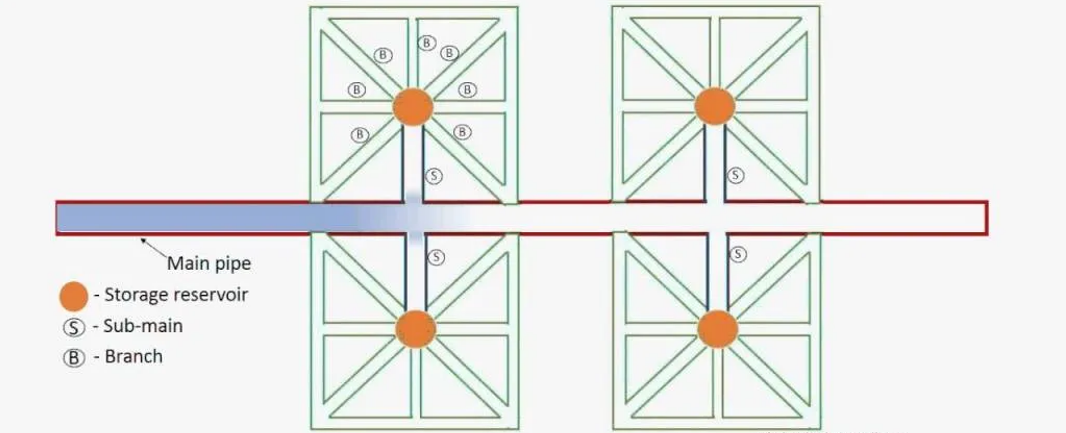
\includegraphics[scale=0.15]{RadialDistributionSystem}\\
    \end{minipage}
    &
  \scriptsize{In this types of water distribution system, the whole buildings are divided into several distribution areas. Each building has a centrally located elevated reservoir from where distribution pipes run radially towards the periphery of the distribution areas.}  
    &
    %\begin{minipage}[t]{5cm}
    \vspace{0.2cm}
      \begin{itemize}[leftmargin=*]
      \scriptsize{
        \item Typically used in high-rise buildings.
        \item Discharge rate is high, low head losses.
        \item Maintenance can be done with minimal flow disruption.
        \item No endpoints, minimal stagnation}
      \end{itemize}
    %\end{minipage}
    & 
    %\begin{minipage}{5cm}
       \begin{itemize}[leftmargin=*]
      \scriptsize{
        \item The design of the pipe laying system is complicated.
        \item More length of pipe is required.}
      \end{itemize}
    %\end{minipage}
    \\ \hline
%\multicolumn{2}{c}{\scriptsize{Grid Iron Distribution System}} & \scriptsize{Advantages} & \scriptsize{Disadvantages}\\ \hline
    \begin{minipage}{.3\textwidth}
        \scriptsize{\textbf{Grid Iron Distribution System}}\\
     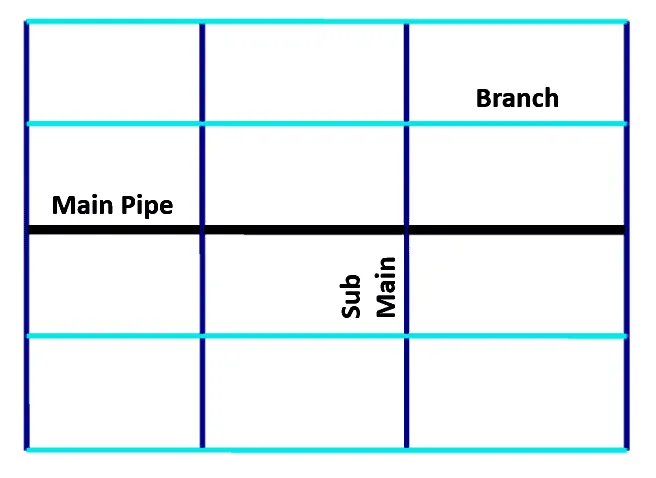
\includegraphics[scale=0.27]{GridIronDistributionSystem}\\
    \end{minipage}
    &
  \scriptsize{Main supply lines run through the center, and sub mains branch off in perpendicular directions. The branch interconnects the sub-mains. All types of pipes are interconnected - no dead ends. Water can reach any given point from many directions, which allows more flexible operation, particularly for repairs.}  
    &
    %\begin{minipage}[t]{5cm}
        \vspace{0.2cm}
      \begin{itemize}[leftmargin=*]
      \scriptsize{
        \item Minimal stagnation or sediment deposit.
        \item Water is available at every point with minimum loss of head.
        \item Water is delivered with adequate pressure for firefighting.
        \item During repair, few houses are affected.}
      \end{itemize}
      \vspace{-1em} 
    %\end{minipage}
    & 
    %\begin{minipage}{5cm}
       \begin{itemize}[leftmargin=*]
      \scriptsize{
        \item In this system, more cut-off valves are required.
        \item This system requires longer pipe lengths with larger diameters.
        \item The analysis of discharge, pressure, and velocity in the pipes is difficult and cumbersome.}
      \end{itemize}
    %\end{minipage}
    \\ \hline
   \end{tabular}
   \caption{Types of Distribution Systems}
   \label{table:TypesofDistributionSystems}
\end{table}

\thispagestyle{empty}

\begin{table}[h!]
  \centering
  \begin{tabular}{| m{5cm} | m{5cm} | m{5cm} | m{5cm}|}
    \hline
    \textbf{Pipe Material} & \textbf{Advantages} & \textbf{Disadvantages} & \textbf{Joints}\\
 
 \scriptsize{Steel:  These are fabricated by rolling the mild steel plates to proper diameter and can be joined by riveting or welding. Steel pipe is coupled by a variety of methods; threaded
couplings, welded couplings, Dresser\texttrademark type couplings, Victaulic\texttrademark  couplings, flanges and rubber ring push-on joints.}
&
  \scriptsize{\begin{itemize}[leftmargin=*, topsep=5pt, partopsep=0pt]
  \item Numbers of joints are less because these are available in long lengths.

  \item The pipes are cheap at the first cost.

  \item The pipes are durable and strong enough to resist high.

  \item The pipes are flexible to some extent laid on curves. and they can therefore 5. Transportation is easy because of lightweight.
  \end{itemize}}  
    &
  \scriptsize{\begin{itemize}[leftmargin=*, topsep=5pt, partopsep=0pt]
  \item Maintenance cost is high.

  \item The pipes are likely to be rusted by acidic or alkaline water.

  \item The pipes require more time for repairs during breakdown and hence are not suitable for distribution pipes.
  \end{itemize}}  
  & \scriptsize{Steel pipe is coupled by a variety of methods; threaded
couplings, welded couplings, Dresser\texttrademark type couplings, Victaulic\texttrademark couplings, flanges and rubber ring push-on joints.}
    \\ \hline
    
    
    
        \scriptsize{\begin{itemize}[leftmargin=*, topsep=5pt, partopsep=0pt]\item Polyvinyl chloride (PVC) \item Cross linked PVC (CPVC) \end{itemize}}
&
  \scriptsize{\begin{itemize}[leftmargin=*, topsep=5pt, partopsep=0pt]
  \item Cost of these pipes is moderate.

  \item Pipes are cheap and durable.

\item The pipes are flexible, light in weight and they can easy to mold any shape.

\item Does not corrode, tuberculate or support bacteria growth like metal pipe.

  \end{itemize}}  
    &
  \scriptsize{\begin{itemize}[leftmargin=*, topsep=5pt, partopsep=0pt]
  \item The co-efficient of expansion for plastic is high.

\item It is difficult to obtain plastic pipes of uniform composition.

\item The pipes are less resistant to heat.

\item Some pipes of plastic impart taste to the water.
  \end{itemize}} 
  & \scriptsize{PVC Class and Pressure pipe can be connected using either an integral bell and spigot process or a double ended bell. In either case the gasket is a rubber material and the joints
are made by lubricating the pipe and pushing it into the coupling or bell.}
    \\ \hline
    
    
    
    \scriptsize{Ductile iron (DI): Typically, the pipe is manufactured using centrifugal casting in metal or resin-lined molds. Protective internal linings and external coatings are done to ductile iron pipes to overcome corrosion problems.}
&
  \scriptsize{\begin{itemize}[leftmargin=*, topsep=5pt, partopsep=0pt]
  \item Comparatively DI pipes possess greater ductility and impact resistance than CI pipes.

\item Lighter than CI pipes so that easy to handle and transport.

\item The pipes are easy to join and simple also can accommodate some angular deflection.

\item These pipes are of more strength than CI pipes.
  \end{itemize}}  
    &
  \scriptsize{\begin{itemize}[leftmargin=*, topsep=5pt, partopsep=0pt]
  \item The pipes require internal and external lining or protection.

\item Corrosion may take place as equal in CI pipes.

\item The polyethylene wrappings may cause damage. 
  \end{itemize}}  
  
  & \scriptsize{Ductile cast iron pipe is commonly connected using
mechanical joints (M.J.), flanges or the various common rubber ring push-on joints. Fittings used are commonly made of gray or ductile cast iron and use M.J. or hub joints. Service taps are made by directly tapping the line or using service saddles.}
    \\ \hline
    
  
        \scriptsize{Concrete Pipe: Cement concrete pipe pipes may be either plain cement or reinforced cement concrete. PCC pipes can be used up to 15 m head whereas RCC pipes can be used up to the head of 60 in and for higher head pre-stressed concrete can be used.}
&
  \scriptsize{\begin{itemize}[leftmargin=*, topsep=5pt, partopsep=0pt]
  \item There are pipes that are most durable with usual life of about 75 years.

\item The pipes can be cast at site work and thus there is the reduction in transport charges.

\item Maintenance cost is less.

\item Inside surface of the pipe can be made smooth.

\item  No danger of rusting.
  \end{itemize}}  
    &
  \scriptsize{\begin{itemize}[leftmargin=*, topsep=5pt, partopsep=0pt]
  \item Transportation is difficult.

\item Repair work is difficult.

\item Initial cost is high.

\item These pipes are affected by acids, alkalies, and salty waters.
  \end{itemize}}  
  & \scriptsize{This pipe is connected by bell and spigot rubber ring pushon joints. Once the
joint has been connected the exposed steel must be coated with concrete to protect the steel cylinder from corrosion.}
    \\ \hline   
        \end{tabular}
        \caption{Pipe Material of Construction - 1 of 2}
   \label{table:PipelineMaterial1}
    \end{table}   
    
    
    \begin{table}[h!]
  \begin{tabular}{|c m{20cm} |}
    \hline
\multicolumn{2}{c}{Air Gap}\\ \hline
    \begin{minipage}{.3\textwidth}
    \hspace{1cm}
%    \tcbox[colframe=green!30!black,
%           colback=green!30]{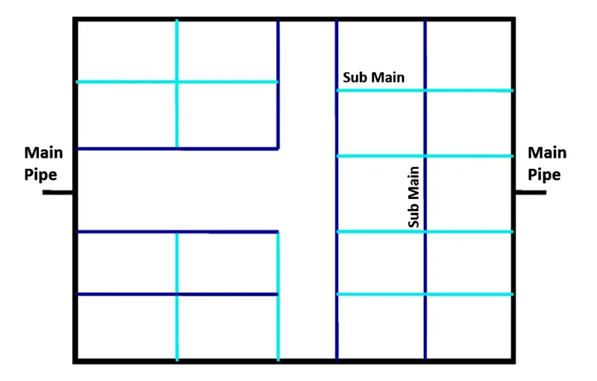
\includegraphics[scale=0.5]{RingDistributionSystem}}    
     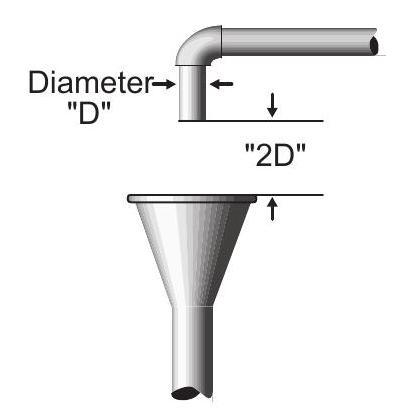
\includegraphics[scale=0.16]{AirGap}\\
    \end{minipage}
     &
    \vspace{0.3cm}
    %\begin{minipage}[t]{5cm}
\scriptsize{\begin{itemize}[topsep=5pt, partopsep=0pt]
\item A physical separation between the free-flowing discharge end of a potable water supply pipeline and an open or non-pressure receiving vessel. 
\item Should not be used in an area with dangerous atmosphere.
\item An "approved air gap" shall be at least twice the diameter of the supply pipe measured vertically above the overflow rim of the receiving vessel; in no case less than 1 inch $(2.54 \mathrm{~cm})$.

\textbf{Common Applications - Lethal hazards (raw sewage, recycled water, auxiliary water supply}
\end{itemize}}
\\ \hline

\multicolumn{2}{c}{Atmospheric Vacuum Breaker Assembly (AVB)}\\ \hline
    \begin{minipage}{.3\textwidth}
%    \tcbox[colframe=green!30!black,
%           colback=green!30]{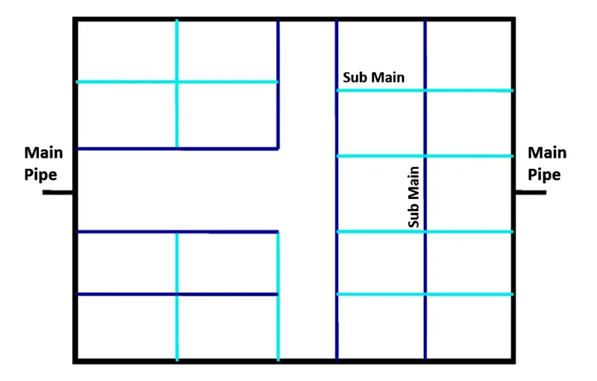
\includegraphics[scale=0.5]{RingDistributionSystem}}    
     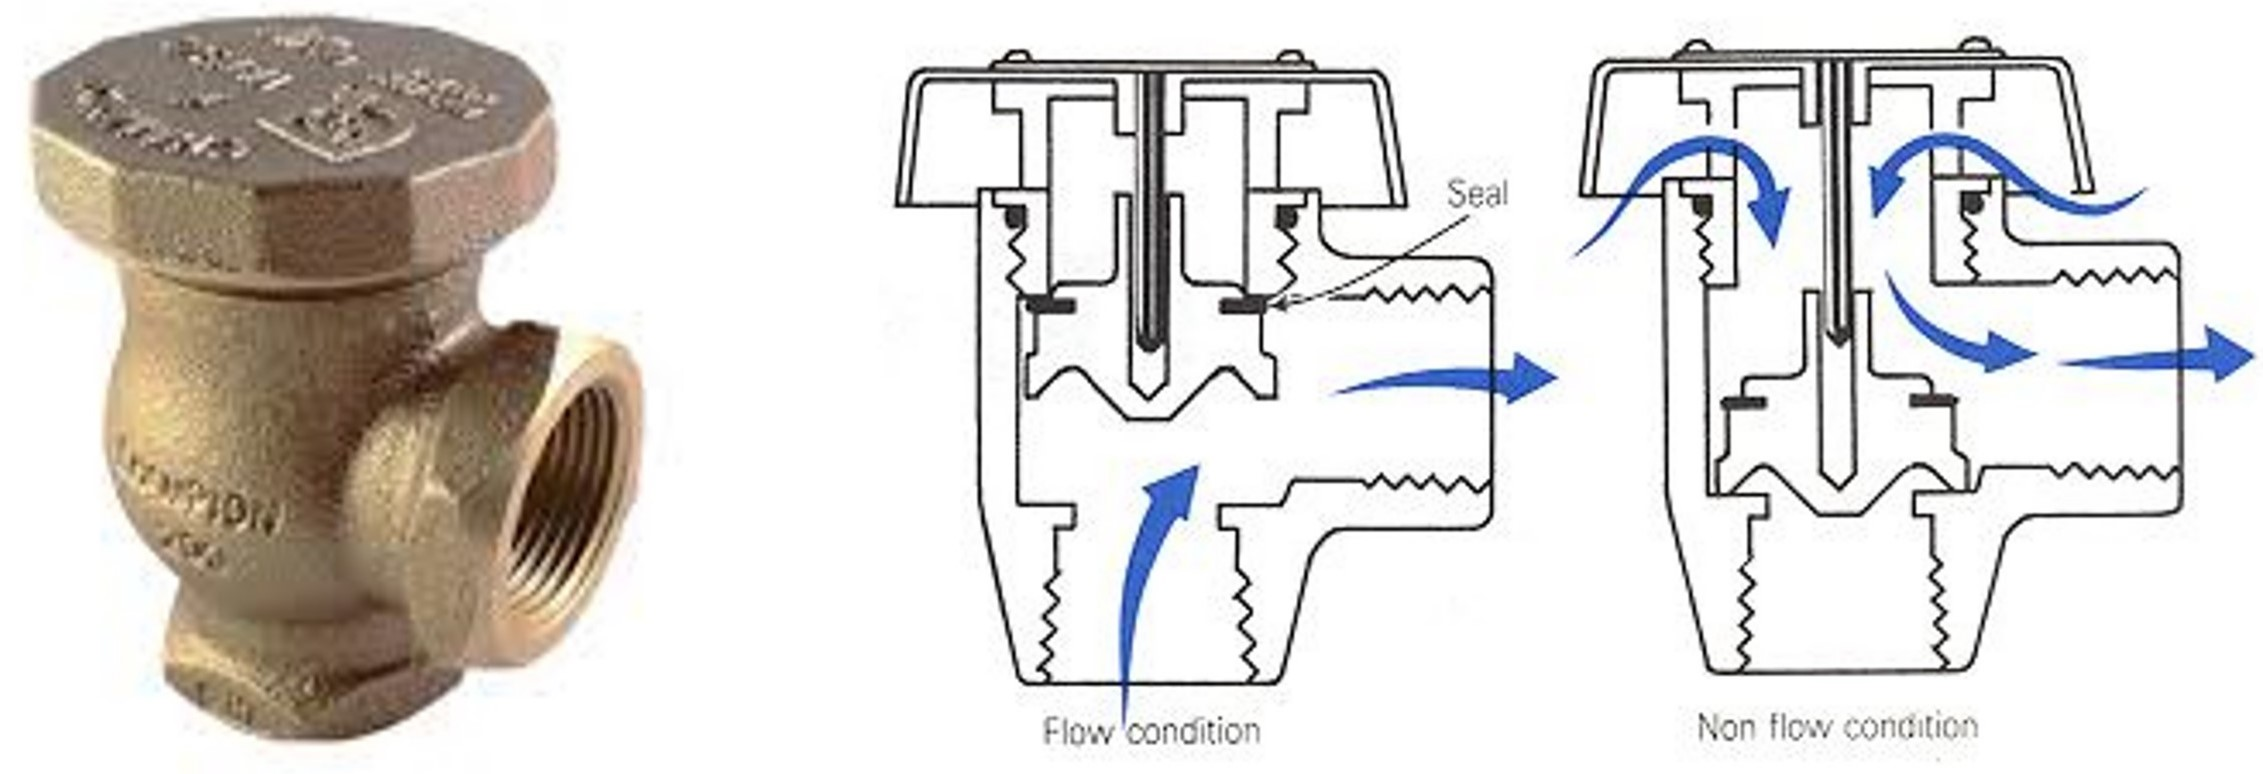
\includegraphics[scale=0.29]{AtmosphericVacuumBreaker(3)}\\
    \end{minipage}
     &
    \vspace{0.3cm}
    %\begin{minipage}[t]{5cm}
\scriptsize{\begin{itemize}[topsep=5pt, partopsep=0pt]
\item Also known as the non-pressure type vacuum breaker, it consists of an air inlet valve, a check seat and an air inlet port(s). (.) The flow of water into the body causes the air inlet valve to close the air inlet port(s). 
\item When the flow of water stops the air inlet valve falls and forms a check valve against backsiphonage. At the same time it opens the air inlet port(s) allowing air to enter and satisfy the vacuum. 
\item A shutoff valve immediately upstream may be an integral part of the assembly, but there shall be no shutoff valves or obstructions downstream. 
\item An atmospheric vacuum breaker is designed to protect against a non-health hazard (i.e., pollutant) or a health hazard (i.e., contaminant) under a back-siphonage condition only.

\textbf{Common Applications - Irrigation systems}


\end{itemize}}
    %\end{minipage}
    
    \\ \hline
\multicolumn{2}{c}{Spill Resistant Vacuum Breaker}\\ \hline
    \begin{minipage}{.3\textwidth}
%    \tcbox[colframe=green!30!black,
%           colback=green!30]{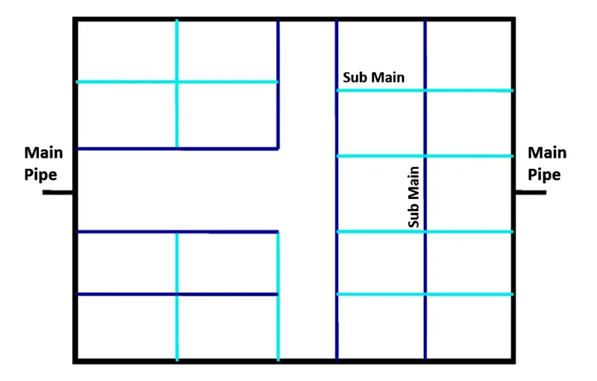
\includegraphics[scale=0.5]{RingDistributionSystem}}    
     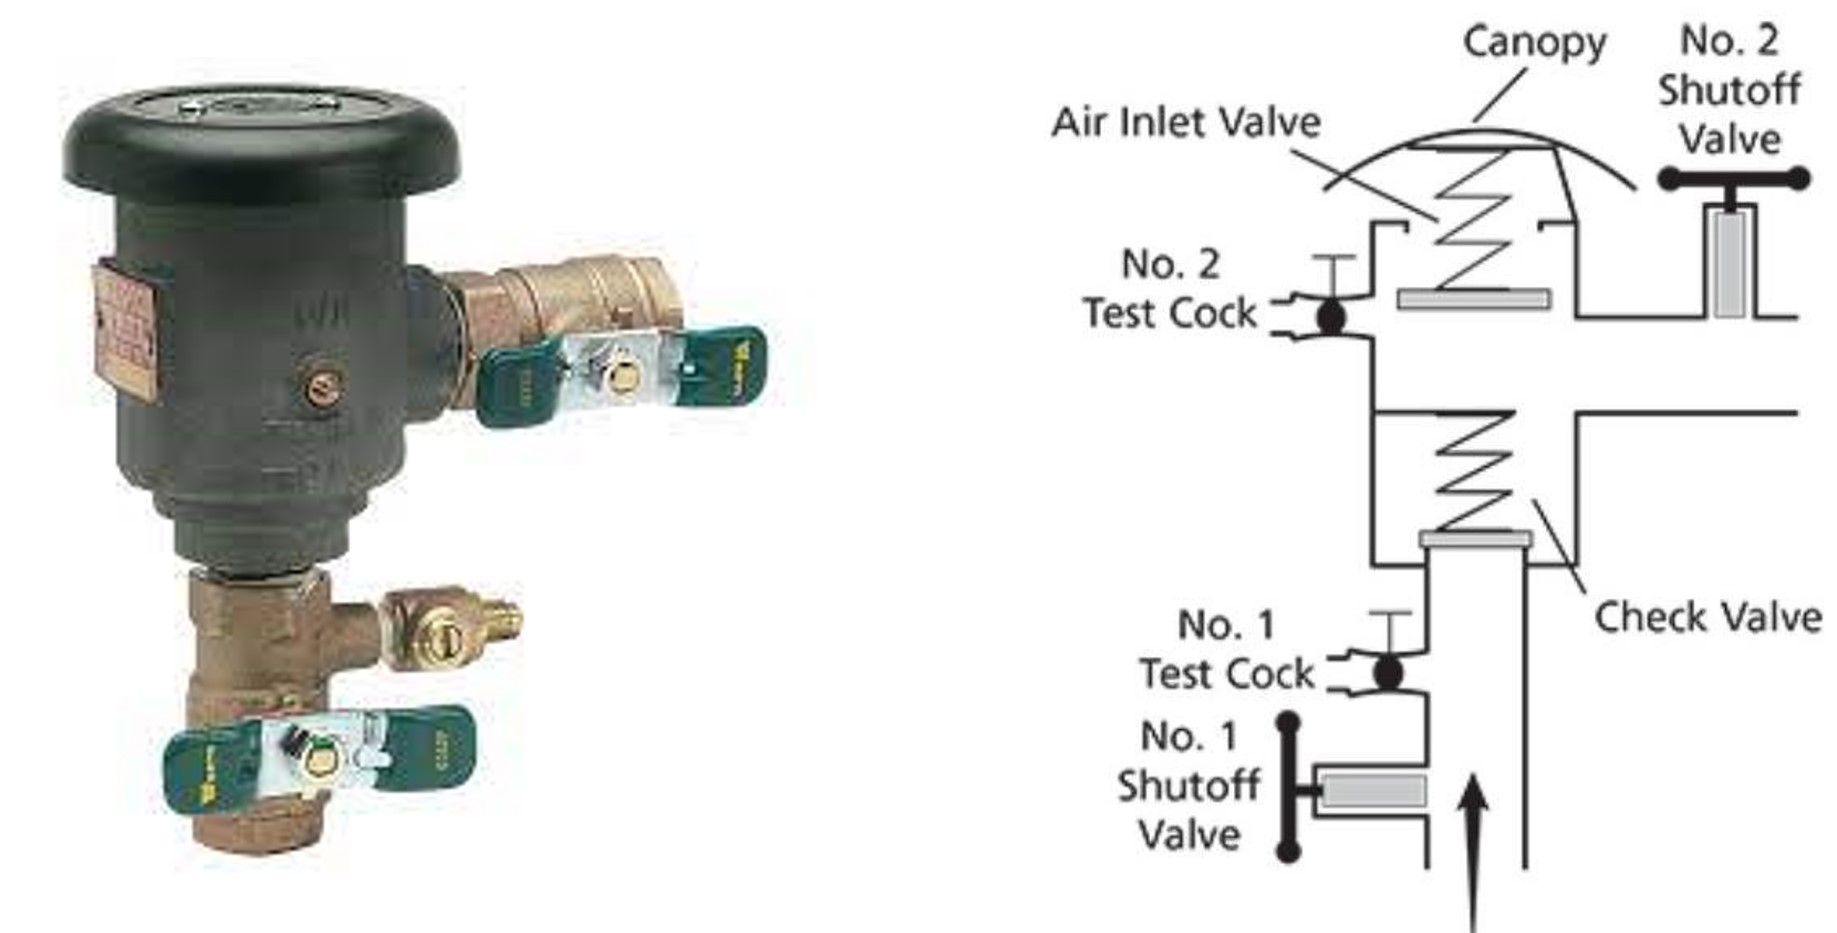
\includegraphics[scale=0.38]{SpillResitantVacuumBreaker1}\\
    \end{minipage}
     &
    \vspace{0.4cm}
    %\begin{minipage}[t]{5cm}
 \scriptsize{\begin{itemize}[topsep=5pt, partopsep=0pt]
\item Its assembly consists of an independently operating internally loaded check valve and independently operating loaded air inlet valve located on the discharge side of the check valve. 
\item The assembly is to be equipped with a properly located resilient seated test cock, a properly located bleed/vent port, and tightly closing resilient seated shutoff valves attached at each end of the assembly. 
\item This assembly is designed to protect against a non-health hazard(i.e., pollutant) or a health hazard (i.e., contaminant) under a backsiphonage condition only.

\textbf{Common Applications - Irrigation systems}
\end{itemize}}
\\ \hline

\multicolumn{2}{c}{Swing Check Valve}\\ \hline
    \begin{minipage}{.3\textwidth}
%    \tcbox[colframe=green!30!black,
%           colback=green!30]{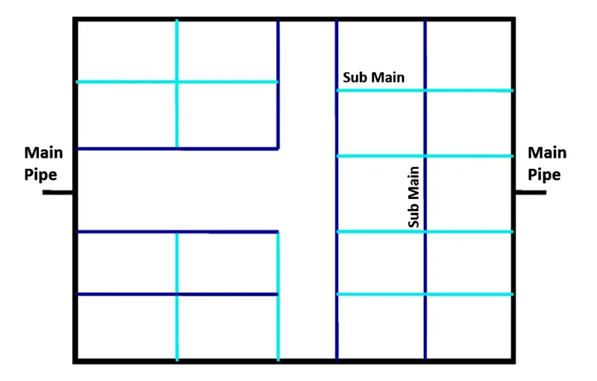
\includegraphics[scale=0.5]{RingDistributionSystem}}    
     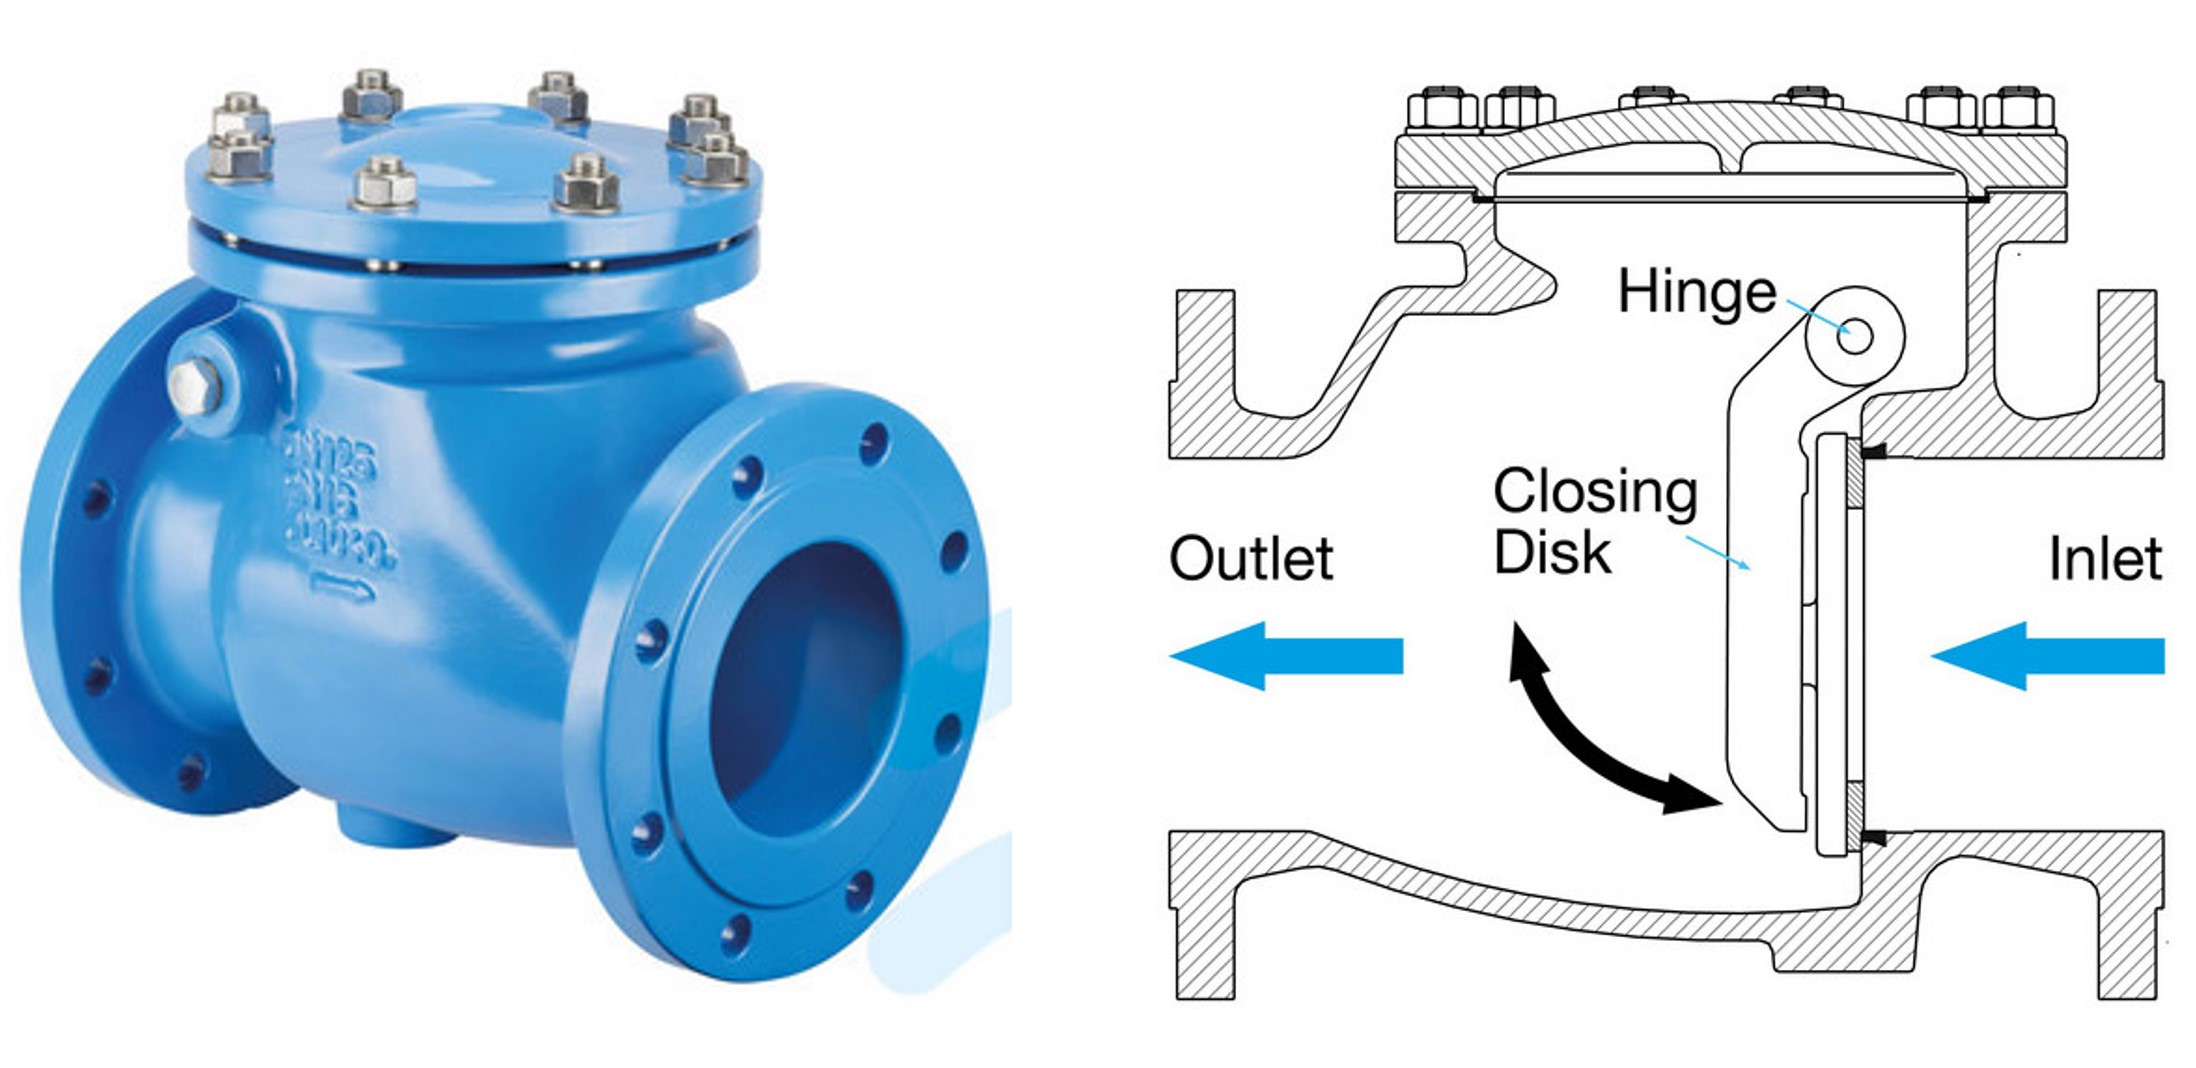
\includegraphics[scale=0.3]{SwingCheckValve1}\\
    \end{minipage}
     &
    \vspace{0.4cm}
    %\begin{minipage}[t]{5cm}
 \scriptsize{\begin{itemize}[topsep=5pt, partopsep=0pt]
\item Its assembly consists of an independently operating internally loaded check valve and independently operating loaded air inlet valve located on the discharge side of the check valve. 
\item The assembly is to be equipped with a properly located resilient seated test cock, a properly located bleed/vent port, and tightly closing resilient seated shutoff valves attached at each end of the assembly. 
\item This assembly is designed to protect against a non-health hazard(i.e., pollutant) or a health hazard (i.e., contaminant) under a backsiphonage condition only.

\textbf{Common Applications - Irrigation systems}
\end{itemize}}
\\ \hline
    %\end{minipage}
\end{tabular}
\caption{Backflow prevention devices - Table 1 of 2}  
                \label{table:Backflow1} 
\end{table}

\begin{table}[h!]
\begin{tabular}{|p{2cm}|p{5.5cm}|p{5.5cm}|}
\hline
%\multicolumn{1}{|c|}{\textbf{CLASSIFICATION}} & \multicolumn{1}{c|}{\textbf{MATERIAL INVOLVED}}                                                                                                                                                                                                                                             & \multicolumn{1}{c|}{\textbf{METHODS FOR EXTINGUISHING \\SMALL   FIRES}}                                                                                                                                                                                       \\ \hline
CLASS & MATERIAL INVOLVED & MEASURES TO FIGHT SMALL FIRES \\ \hline

CLASS A                                       & This class of fire involves ordinary combustibles  or fibrous material, such as wood, paper, cloth, paper, and some plastics.                                                                                                                                                               & Extinguish with pressurized   water, foam, or multipurpose dry chemical extinguishers. Do not use carbon   dioxide or ordinary dry chemical extinguishers on Class A fires.                                                                                \\ \hline
CLASS B                                       & Class B fire is flammable or   combustible liquids such as gasoline, diesel, kerosene, paint, paint   thinners, and propane.                                                                                                                                                                & Extinguish Class B fires by   removing oxygen, by preventing vapors from reaching ignition sources, or by   inhibiting the chemical chain reaction. Use foam, carbon dioxide, ordinary   dry chemical, multipurpose dry chemical, and halon extinguishers. \\ \hline
CLASS C                                       & A Class C fire is energized   electrical equipment, such as motors, motor controls, switches panel boxes,   and power tools.                                                                                                                                                                & Extinguish Class C fires by   using carbon dioxide, ordinary dry chemical, multipurpose dry chemical, and   halon-free extinguishers.                                                                                                                      \\ \hline
CLASS D                                       & A Class D fire is certain   combustible metals, such as magnesium, titanium, potassium, and sodium. These   metals bum at high temperatures and give off sufficient oxygen to support   combustion. They may react violently with water or other chemicals and must be   handled with care. & Extinguish Class D fires by   using dry powder extinguishers made especially for this type of fire                                                                                                                                                         \\ \hline
\end{tabular}
\caption{Fires Classifications}\index{Fires class/classifications}
\end{table}

\begin{table}[h!]    
\begin{center}
     \begin{tabular}{ | m{5cm}  m{5cm} |}
     \hline
           \multicolumn{1}{|c}{} & \multicolumn{1}{c|}{} \\
      \multicolumn{1}{|c}{\textbf{METAL ION (CATION)}} & \multicolumn{1}{c|}{\textbf{NON-METAL ION (ANION)}} \\
            \multicolumn{1}{|c}{} & \multicolumn{1}{c|}{}\\
      Calcium - Ca$^{+2}$ & Carbonate - CO$_3^{\enspace -1}$\\
      Magnesium - Mg$^{+2}$ & Bicarbonate - HCO$_3^{\enspace -1}$\\
      Manganese - Mn$^{+2}$ & Hydroxide - OH$^{-1}$\\
      Iron - Fe$^{+2/+3}$ & Sulfate - SO$_4^{\enspace -2}$\\
      Aluminum - Al$^{+3}$ & Chloride - Cl$^{-1}$\\
      Sodium - Na$^{+1}$ & \\
      Copper - Cu$^{+2/+3}$ & \\
          \hline
                    \end{tabular}
     \caption{Salts constituents}
     \label{Salts constituents}\index{Salts constituents}
     
\end{center}
     \end{table}
     
     
     
     \begin{table}[h!]    
\begin{center}
     \begin{tabular}{ | m{5cm}  m{4cm}  m{4cm} |}
     \hline
           \multicolumn{1}{|c}{} & \multicolumn{1}{c}{} & \multicolumn{1}{c|}{}\\
      \multicolumn{1}{|c}{\textbf{CHEMICAL NAME}} & \multicolumn{1}{c}{\textbf{FORMULA}} & \multicolumn{1}{c|}{\textbf{COMMON NAME}}\\
            \multicolumn{1}{|c}{} & \multicolumn{1}{c}{} & \multicolumn{1}{c|}{}\\
      Aluminum sulfate & Al$_2$(SO$_4$)$_3$ & Alum\\
      Calcium oxide & Ca$ $O$ $ $ $ & Quicklime\\
      Calcium hydroxide & Ca$ $(OH$ $)$_2$ & Slaked/hydrated lime\\
      Calcium carbonate & Ca$ $CO$_3$ $ $ & Limestone\\
      Calcium hydroxide & Ca$ $(OH$ $)$_2$ & Slaked/hydrated lime\\
      Magnesium carbonate & Mg$ $(CO$_3$)$_2$ & \\
      Magnesium bicarbonate & Mg$ $(HCO$_3$)$_2$ & \\
      Sodium hydroxide & Na$ $OH$ $ $ $ & Caustic soda\\
      Sodium carbonate & Na$_2$CO$_3$ $ $ & Soda ash\\
      Ferrous sulfate & Fe$ $SO$_4$ $ $ & Copperas \\
      Ferric chloride & Fe$ $Cl$_3$ $ $ & \\
      Ferrous chloride & Fe$ $Cl$_2$ $ $ & \\
      Copper sulfate & Cu$ $SO$_4$ $ $ &\\

          \hline
                    \end{tabular}
     \caption{Salts found in water and/or used in water treatment}
     \label{Salts found in water and/or used in water treatment}\index{Salts found in water and/or used in water treatment}
     
\end{center}
     \end{table}
     
     \begin{table}[h!]
\begin{tabular}{|p{4cm}|p{3cm}|p{4cm}|p{3cm}|}
\hline
\multicolumn{1}{|c|}{\textbf{Parameter}}                                                   & \multicolumn{1}{c|}{\textbf{Container}}                                            & \multicolumn{1}{c|}{\textbf{Preservative}}                                                                                                                   & \multicolumn{1}{c|}{\textbf{Holding Time}}                          \\ \hline
\begin{tabular}[c]{@{}l@{}}Coliform, Total or Fecal,\\      Chlorinated Water\end{tabular} & \begin{tabular}[c]{@{}l@{}}Sterile Container    w/\\      thiosulfate\end{tabular} & Cool   to \textless{}10 °C.  Do not freeze                                                                                                                    & 8   hrs for source water compliance and 30 hours for drinking water \\ \hline
Giardia and   Cryptosporidium                                                              & 10   L plastic container                                                           & Cool   to \textless{}10  °C .  Do not freeze                                                                                                                    & 96   hours                                                          \\ \hline
Alkalinity, Turbidity, Solids                                                             , Fluoride & Plastic or Glass                                                                   & Cool   to \textless{} 4 °C                                                                                                                                             & Method   dependent                                                  \\ \hline
Metals, General                                                                            & Plastic or Glass, Rinsed w/ 1:1 HNO3                                               & Nitric   acid to pH \textless 2                                                                                                                              & 6 Months                                                            \\ \hline
Hardness, Total                                                                            & Plastic or Glass                                                                   & Nitric   acid to pH \textless 2                                                                                                                              & 6 Months                                                            \\ \hline
pH                                                                                         & Plastic or Glass                                                                   & None                                                                                                                                                         & Analyze in 15 min                                                    \\ \hline
Nitrogen and   phosphorous compounds                                                       & Plastic or Glass                                                                   & Sulfuric acid to   pH\textless{}2                                                                                                                            & 28 days                                                             \\ \hline
VOCs, TTHMs                                                                                & Glass bottle                                                                       & Sodium thiosulfate or   Ascorbic acid if sample chlorinated and Hydrochloric Acid (HCl) to pH \textless 2  and cool to  \textless 4 °C  but do not freeze & 14 days                                                             \\ \hline
\end{tabular}
\caption*{Key Parameters Sampling Requirements}
\end{table}
\newpage
\begin{table}[ht]
\begin{center}
\begin{tabular}{|l|l|llll}
\hline
\multirow{9}{*}{Fresh water} & \multirow{9}{*}{2.50\%} & \multicolumn{1}{l|}{\multirow{7}{*}{Surface water}} & \multicolumn{1}{l|}{\multirow{7}{*}{1.20\%}} & \multicolumn{1}{l|}{Atmosphere}                & \multicolumn{1}{l|}{3.00\%}  \\ \cline{5-6} 
                             &                         & \multicolumn{1}{l|}{}                               & \multicolumn{1}{l|}{}                        & \multicolumn{1}{l|}{Living things}             & \multicolumn{1}{l|}{0.26\%}  \\ \cline{5-6} 
                             &                         & \multicolumn{1}{l|}{}                               & \multicolumn{1}{l|}{}                        & \multicolumn{1}{l|}{Rivers}                    & \multicolumn{1}{l|}{0.49\%}  \\ \cline{5-6} 
                             &                         & \multicolumn{1}{l|}{}                               & \multicolumn{1}{l|}{}                        & \multicolumn{1}{l|}{Swamps, marshes}           & \multicolumn{1}{l|}{2.60\%}  \\ \cline{5-6} 
                             &                         & \multicolumn{1}{l|}{}                               & \multicolumn{1}{l|}{}                        & \multicolumn{1}{l|}{Soil moisture}             & \multicolumn{1}{l|}{3.80\%}  \\ \cline{5-6} 
                             &                         & \multicolumn{1}{l|}{}                               & \multicolumn{1}{l|}{}                        & \multicolumn{1}{l|}{Lakes}                     & \multicolumn{1}{l|}{20.90\%} \\ \cline{5-6} 
                             &                         & \multicolumn{1}{l|}{}                               & \multicolumn{1}{l|}{}                        & \multicolumn{1}{l|}{Ground ice and permafrost} & \multicolumn{1}{l|}{69.00\%} \\ \cline{3-6} 
                             &                         & \multicolumn{1}{l|}{Ground water}                   & \multicolumn{1}{l|}{30.10\%}                 &                                                &                              \\ \cline{3-4}
                             &                         & \multicolumn{1}{l|}{Glaciers and ice caps}          & \multicolumn{1}{l|}{68.70\%}                 &                                                &                              \\ \cline{1-4}
Other saline   water         & 0.90\%                  &                                                     &                                              &                                                &                              \\ \cline{1-2}
Oceans                       & 96.50\%                 &                                                     &                                              &                                                &                              \\ \cline{1-2}
\end{tabular}
\caption{Distribution of Earth's Water}
\textit{(From:  Igor Shiklomanov's chapter "Worlds fresh water resources" in Peter H. Gleick (editor), \\1993, Water in Crisis: A guide to the world's Fresh water resources)}
\end{center}
\end{table}     

\newpage

\begin{table}[ht]
\begin{tabular}{|l|l|l|l|l|}
\hline
\multicolumn{1}{|c|}{\textbf{Name}} & \multicolumn{1}{c|}{\textbf{Power}} & \multicolumn{1}{c|}{\textbf{Number}} & \multicolumn{1}{c|}{\textbf{SI symbol}} & \multicolumn{1}{c|}{\textbf{SI prefix}} \\ \hline
one                                 & $10^0$& 1                                    &                                         &                                         \\ \hline
ten                                 & $10^1$                                   & 10                                   & da (D)                                  & deca                                    \\ \hline
hundred                             & $10^2$                                   & 100                                  & h (H)                                   & hecto                                   \\ \hline
thousand                            & $10^3$                                  & 1,000                                & k (K)                                   & kilo                                    \\ \hline
million                             & $10^6$                                   & 1,000,000                            & M                                       & mega                                    \\ \hline
billion                             & $10^9$                                  & 1,000,000,000                        & G                                       & giga                                    \\ \hline
tenth                               & $10^{-1}$                                 & 0.1                                  & d                                       & deci                                    \\ \hline
hundredth                           & $10^{-2}$                                  & 0.01                                 & c                                       & centi                                   \\ \hline
thousandth                          & $10^{-3} $                                 & 0.001                                & m                                       & milli                                   \\ \hline
millionth                           &$10^{-6} $                               & 0.000 001                            & $\mu$                                      & micro                                   \\ \hline
billionth                           & $10^{-9} $                               & 0.000 000 001                        & n                                       & nano                                    \\ \hline
\end{tabular}
\end{table}

\newpage
\begin{table}[h]
\begin{tabular}{|p{16cm}|}
\hline
\scriptsize{1000 has   one significant digit: only the 1 is interesting (only it tells us anything   specific); we don't know anything for sure about the hundreds, tens, or units   places; the zeroes may just be placeholders; they may have rounded something   off to get this value.                                    } \\ \hline
\scriptsize{1000.0 has five significant   digits: the ".0" tells us something interesting about the presumed   accuracy of the measurement being made; namely, that the measurement is   accurate to the tenths place, but that there happen to be zero tenths.                                                               } \\ \hline
\scriptsize{0.00035 has two significant   digits: only the 3 and 5 tell us something; the other zeroes are   placeholders, only providing information about relative size.                                                                                                                                                    } \\ \hline
\scriptsize{0.000350 has three significant   digits: the last zero tells us that the measurement was made accurate to that   last digit, which just happened to have a value of zero.                                                                                                                                         } \\ \hline
\scriptsize{1006 has four significant   digits: the 1 and 6 are interesting, and we have to count the zeroes, because   they're between the two interesting numbers.                                                                                                                                                          } \\ \hline
\scriptsize{560 has two significant   digits: the last zero is just a placeholder.                                                                                                                                                                                                                                            } \\ \hline
\scriptsize{560. : notice that   "point" after the zero! This has three significant digits, because   the decimal point tells us that the measurement was made to the nearest unit,   so the zero is not just a placeholder.                                                                                                  } \\ \hline
\scriptsize{560.0 has four significant   digits: the zero in the tenths place means that the measurement was made   accurate to the tenths place, and that there just happen to be zero tenths;   the 5 and 6 give useful information, and the other zero is between   significant digits, and must therefore also be counted.} \\ \hline
\end{tabular}
\end{table}
\newpage
\begin{table}[h!]
  \centering
\small
\begin{tabular}{|lllll|}
\hline
\rowcolor[HTML]{CBCEFB} 
\multicolumn{2}{|l|}{\cellcolor[HTML]{CBCEFB}TCR/ Nitrate/Nitrite}                                                   & \multicolumn{1}{l|}{\cellcolor[HTML]{CBCEFB}CWS} & \multicolumn{1}{l|}{\cellcolor[HTML]{CBCEFB}NTNCWS} & TNCWS                      \\ \hline
\multicolumn{2}{|l|}{Sanitary Survey}                                                                                & \multicolumn{1}{l|}{Every 3 years}               & \multicolumn{1}{l|}{Every 5 years}                  & Every 5 years              \\ \hline
\multicolumn{2}{|l|}{Total Coliform Bacteria1}                                                                       & \multicolumn{1}{l|}{Monthly}                     & \multicolumn{1}{l|}{Monthly}                        & Monthly                    \\ \hline
\multicolumn{2}{|l|}{Nitrate (NO$_3$)}                                                                                  & \multicolumn{1}{l|}{Quarterly$^2$}                  & \multicolumn{1}{l|}{Quarterly$^2$}                     & Annually                   \\ \hline
\multicolumn{2}{|l|}{Nitrite (NO$_2$)}                                                                                  & \multicolumn{1}{l|}{1 sample record}             & \multicolumn{1}{l|}{1 sample record}                & 1 sample record            \\ \hline
\rowcolor[HTML]{CBCEFB} 
\multicolumn{2}{|l|}{\cellcolor[HTML]{CBCEFB}Reporting}                                                              & \multicolumn{1}{l|}{\cellcolor[HTML]{CBCEFB}CWS} & \multicolumn{1}{l|}{\cellcolor[HTML]{CBCEFB}NTNCWS} & TNCWS                      \\ \hline
\multicolumn{2}{|l|}{}                                                                                               & \multicolumn{1}{l|}{Continuous or grab samples}  & \multicolumn{1}{l|}{Continuous or grab samples}     & Continuous or grab samples \\ \hline
\multicolumn{2}{|l|}{Turbidity}                                                                                      & \multicolumn{3}{l|}{(Frequency determined by population and   filtration type.)}                                                    \\ \hline
\multicolumn{2}{|l|}{Fluoride – if added}                                                                            & \multicolumn{1}{l|}{Daily}                       & \multicolumn{1}{l|}{Daily}                          &                            \\ \hline
\multicolumn{2}{|l|}{}                                                                                               & \multicolumn{1}{l|}{Continuous or grab samples}  & \multicolumn{1}{l|}{Continuous or grab samples}     & Continuous or grab samples \\ \cline{3-5} 
\multicolumn{2}{|l|}{\multirow{-2}{*}{Entry Point Chlorine – if chlorine is added}}                                  & \multicolumn{3}{l|}{(Pop determines how many times a   day chlorine is measured.)}                                                  \\ \hline
\multicolumn{2}{|l|}{Distribution System Chlorine3}                                                                  & \multicolumn{1}{l|}{Monthly}                     & \multicolumn{1}{l|}{Monthly}                        & Monthly                    \\ \hline
\multicolumn{2}{|l|}{Consumer Confidence Report}                                                                     & \multicolumn{1}{l|}{Annually}                    & \multicolumn{1}{l|}{Annually}                       &                            \\ \hline
\rowcolor[HTML]{CBCEFB} 
\multicolumn{2}{|l|}{\cellcolor[HTML]{CBCEFB}Disinfection/Disinfectant Byproducts}                                   & \multicolumn{1}{l|}{\cellcolor[HTML]{CBCEFB}CWS} & \multicolumn{1}{l|}{\cellcolor[HTML]{CBCEFB}NTNCWS} & TNCWS                      \\ \hline
\multicolumn{1}{|l|}{}                                                      & \multicolumn{1}{l|}{Pop \textless 500} & \multicolumn{1}{l|}{Annually}                    & \multicolumn{1}{l|}{Annually}                       & Annually                   \\ \cline{2-5} 
\multicolumn{1}{|l|}{}                                                      & \multicolumn{1}{l|}{Pop 500 -   9,999} & \multicolumn{1}{l|}{Quarterly}                   & \multicolumn{1}{l|}{Quarterly}                      & Quarterly                  \\ \cline{2-5} 
\multicolumn{1}{|l|}{\multirow{-3}{*}{Total   Trihalomethanes (TTHM/HAA5)}} & \multicolumn{1}{l|}{Pop 10,000}        & \multicolumn{1}{l|}{Quarterly}                   & \multicolumn{1}{l|}{Quarterly}                      & Quarterly                  \\ \hline
\multicolumn{2}{|l|}{TOC and Alkalinity}                                                                             & \multicolumn{1}{l|}{Monthly2}                    & \multicolumn{1}{l|}{Monthly2}                       &                            \\ \hline
\multicolumn{2}{|l|}{Bromate (Ozone plants only)}                                                                    & \multicolumn{1}{l|}{Monthly}                     & \multicolumn{1}{l|}{Monthly}                        &                            \\ \hline
\rowcolor[HTML]{CBCEFB} 
\multicolumn{2}{|l|}{\cellcolor[HTML]{CBCEFB}Inorganic Chemicals}                                                    & \multicolumn{1}{l|}{\cellcolor[HTML]{CBCEFB}CWS} & \multicolumn{1}{l|}{\cellcolor[HTML]{CBCEFB}NTNCWS} & TNCWS                      \\ \hline
\multicolumn{2}{|l|}{All Primary}                                                                                    & \multicolumn{1}{l|}{Annually}                    & \multicolumn{1}{l|}{Annually}                       &                            \\ \hline
\multicolumn{2}{|l|}{Arsenic}                                                                                        & \multicolumn{1}{l|}{Annually}                    & \multicolumn{1}{l|}{Annually}                       &                            \\ \hline
\multicolumn{2}{|l|}{Asbestos}                                                                                       & \multicolumn{1}{l|}{Once per period}             & \multicolumn{1}{l|}{Once per period}                &                            \\ \hline
\multicolumn{2}{|l|}{Lead and Copper1}                                                                               & \multicolumn{1}{l|}{Every 6 months$^2$}             & \multicolumn{1}{l|}{Every 6 months$^2$}                &                            \\ \hline
\rowcolor[HTML]{CBCEFB} 
\multicolumn{2}{|l|}{\cellcolor[HTML]{CBCEFB}Organic Chemicals}                                                      & \multicolumn{1}{l|}{\cellcolor[HTML]{CBCEFB}CWS} & \multicolumn{1}{l|}{\cellcolor[HTML]{CBCEFB}NTNCWS} & TNCWS                      \\ \hline
\multicolumn{2}{|l|}{Pesticides (SOCs) and Other Organics}                                                           & \multicolumn{1}{l|}{Quarterly$^2$}                  & \multicolumn{1}{l|}{Quarterly$^2$}                     &                            \\ \hline
\multicolumn{2}{|l|}{}                                                                                               & \multicolumn{1}{l|}{Quarterly}                   & \multicolumn{1}{l|}{Quarterly}                      &                            \\ \cline{3-5} 
\multicolumn{2}{|l|}{\multirow{-2}{*}{Volatile Organic Chemicals (VOCs)}}                                            & \multicolumn{1}{l|}{Annually}                    & \multicolumn{1}{l|}{Annually}                       &                            \\ \hline
\rowcolor[HTML]{CBCEFB} 
\multicolumn{2}{|l|}{\cellcolor[HTML]{CBCEFB}Radionuclides}                                                          & \multicolumn{1}{l|}{\cellcolor[HTML]{CBCEFB}CWS} & \multicolumn{1}{l|}{\cellcolor[HTML]{CBCEFB}NTNCWS} & TNCWS                      \\ \hline
\multicolumn{2}{|l|}{Gross Alpha Radioactivity}                                                                      & \multicolumn{1}{l|}{Quarterly}                   & \multicolumn{1}{l|}{}                               &                            \\ \hline
\multicolumn{2}{|l|}{Radium 226, Radium 228, Uranium}                                                                & \multicolumn{1}{l|}{Quarterly}                   & \multicolumn{1}{l|}{}                               &                            \\ \hline
\multicolumn{5}{|l|}{1 Number of samples is based   on population. 2 May be   reduced if certain criteria are met.}                                                                                                                                        \\ \hline
\multicolumn{5}{|l|}{3 Distribution point chlorine   test is required at the same time and location as total coliform samples are   collected.}                                                                                                            \\ \hline
\multicolumn{5}{|l|}{Cycle – 3 years; Period – 9 years}                                                                                                                                                                                                    \\ \hline
\end{tabular}
\caption{SWTR sampling and testing schedules for surface water and GUDISW}
%\textit{(Source:Introduction to Small Water Systems - Alaska DEC)}

\end{table}
\newpage
\begin{table}[]
\begin{center}
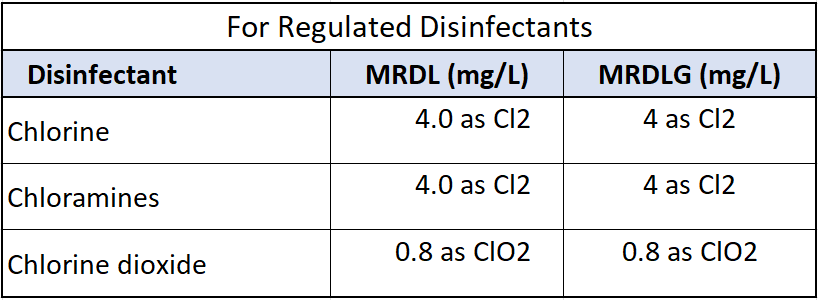
\includegraphics[scale=0.5]{DinfectantMRDLS}
\caption{Disinfectant MRDLs}
\label{table:DisinfectantMRDLs}
\end{center}
\end{table}
\begin{table}[]
\begin{center}
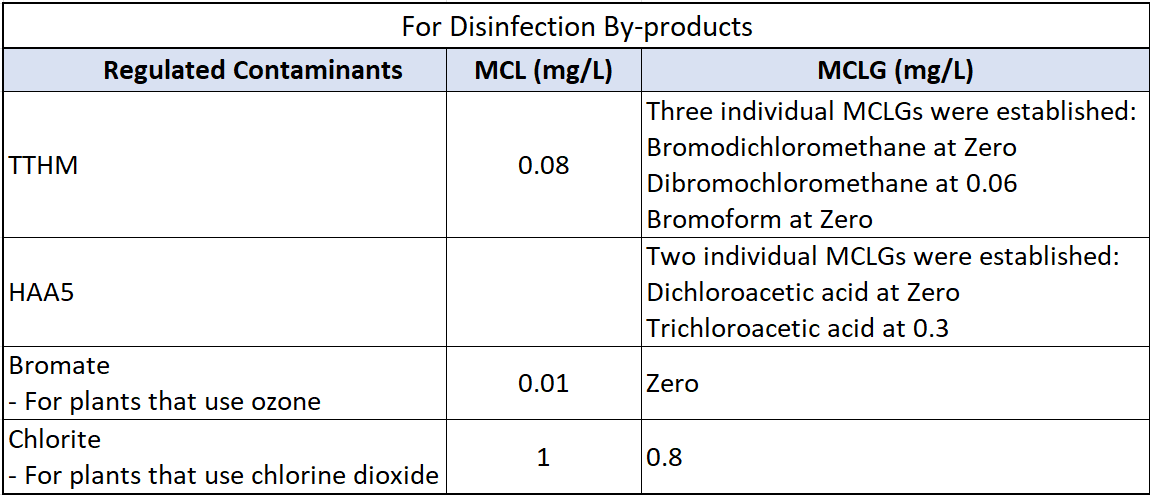
\includegraphics[scale=0.5]{DBPMCLS}
\caption{Disinfectant By-products MCLs}
\label{table:DBPMCL}
\end{center}
\end{table}

\newpage
\begin{table}[H]
\begin{center}
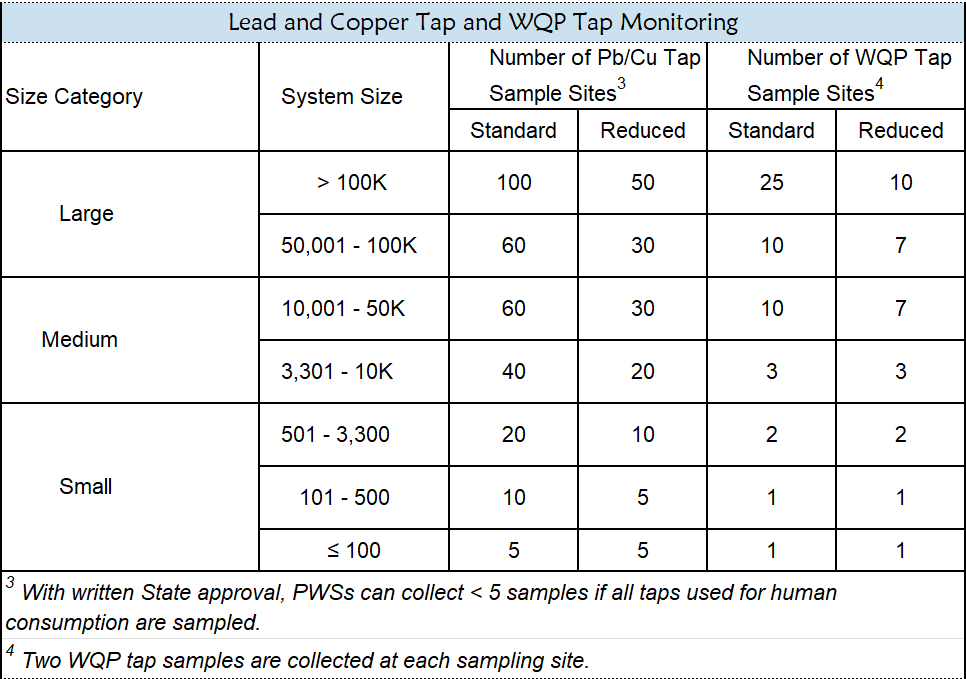
\includegraphics[scale=0.5]{LCRMonitoring}
\caption{Lead and Copper Tap and WQP Tap Monitoring}
\end{center}
\end{table}
\newpage


\begin{table}[h!]
\begin{center}
\begin{tabular}{|l|l|}
\hline
\multicolumn{1}{|c|}{\textbf{Record}} & \multicolumn{1}{c|}{\textbf{Minimum Record   Retention Period}} \\ \hline
Microbiological   analyses            & 5 years                                                         \\ \hline
Turbidity   analyses                  & 5 years                                                         \\ \hline
Chemical   analyses                   & 10 years                                                        \\ \hline
Sanitary   survey documents           & 10 years                                                        \\ \hline
Variances and   exemptions granted    & 5 years                                                         \\ \hline
Tier 1, Tier 2   and Tier 3 Notices   & 3 years                                                         \\ \hline
Level 1 and   Level 2 assessments     & 5 years                                                         \\ \hline
\end{tabular}
\caption{Summary of regulatory record-keeping requirements}
\end{center}
\end{table}

\newpage

\begin{table}[h!]


\begin{tabular}{p{2cm}p{2.5cm}p{2.5cm}p{2.5cm}p{2.5cm}|}
\hline
\multicolumn{5}{|c|}{\textbf{Inorganics}}                                                                                                                                                                                                                                                                             
 \\ \hline
\multicolumn{1}{|p{2.5cm}|}{} & 
\multicolumn{1}{p{2.5cm}|}{\textbf{With waiver}} & 
\multicolumn{1}{p{2.5cm}|}{\textbf{$\le$ MCL and no waiver}} & 
\multicolumn{1}{p{2.5cm}|}{\textbf{Reliably   and consistently \textless MCL}} & 
\multicolumn{1}{p{2.5cm}|}{\textbf{\textgreater   MCL or not Reliably and consistently \textless MCL}} 
\\ \hline

\multicolumn{1}{|p{2.5cm}|}{Surface water}           & 
\multicolumn{1}{p{2.5cm}|}{Once every 10 years}  & 
\multicolumn{1}{p{2.5cm}|}{Annual}                                     & 
\multicolumn{1}{p{2.5cm}|}{Annual}                                               & 
\multicolumn{1}{p{2.5cm}|}{Quarterly at each   EPTDS}                                                     
\\ \hline



\multicolumn{1}{|p{2.5cm}|}{Ground water}            &
\multicolumn{1}{p{2.5cm}|}{Once every 10 years}  & 
\multicolumn{1}{p{2.5cm}|}{Triennial}                                   & 
\multicolumn{1}{p{2.5cm}|}{Triennial}  & 
\multicolumn{1}{p{2.5cm}|}{Quarterly at each   EPTDS}              
\\ \hline
\end{tabular}


\begin{tabular}{p{1.5cm}p{2.1cm}p{2.1cm}p{2.1cm}p{2.1cm}p{2.1cm}|}
\hline
\multicolumn{6}{|c|}{\textbf{Volatile Organic Compounds (VOCs)}}                                                                                                                                                                                                                                                                              \\ \hline
\multicolumn{1}{|p{1.5cm}|}{} 
& \multicolumn{1}{p{2.1cm}|}{\textbf{Waiver with vulnerability analysis}} 
& \multicolumn{1}{p{2.1cm}|}{\textbf{\textless Detect and no waiver}} 
& \multicolumn{1}{p{2.1cm}|}{\textbf{\textless Detect after at least three annual samples}} 
& \multicolumn{1}{p{2.1cm}|} {\textbf{Reliably and consistently \textless MCL} }
& \multicolumn{1}{p{2.1cm}|}{\textbf{$\ge$Detect  not Reliably and consistently \textless MCL}} \\ \hline

\multicolumn{1}{|p{1.5cm}|}{Surface water}           
& \multicolumn{1}{p{2.1cm}|}{Once every 10 years}  
& \multicolumn{1}{p{2.1cm}|}{Annual}                                     
& \multicolumn{1}{p{2.1cm}|}{Triennial}                                               
& \multicolumn{1}{p{2.1cm}|} {Annual}
& \multicolumn{1}{p{2.1cm}|}{ Quarterly } \\ \hline

\multicolumn{1}{|p{1.5cm}|}{Ground water}            
& \multicolumn{1}{p{2.1cm}|}{Once every 10 years}  
& \multicolumn{1}{p{2.1cm}|}{Annual}                                   
& \multicolumn{1}{p{2.1cm}|}{Annual}   
& \multicolumn{1}{p{2.1cm}|} {Annual}  
& \multicolumn{1}{p{2.1cm}|} {Quarterly} 
\\ \hline
\end{tabular}


\begin{tabular}{
p{3.225cm}
p{3.225cm}
p{3.225cm}
p{3.225cm}|}
\hline

\multicolumn{4}{|c|}{\textbf{Synthetic Organic Compounds (SOCs)}}                                                                                                                                                                                                                                                                              \\ \hline

\multicolumn{1}{|p{3.225cm}|}{\textbf{Reliably and consistently \textless MCL}} & 
\multicolumn{1}{p{3.225cm}|}{\textbf{\textgreater   Detect or not Reliably and consistently \textless MCL}} &
\multicolumn{1}{p{3.225cm}|}{\textbf{Waiver with Vulnerability Assessment every three years}} & 
\multicolumn{1}{p{3.225cm}|}{\textbf{\textless Detect and no waiver}}
\\ \hline

\multicolumn{1}{|p{3.225cm}|}{Annual}  & 
\multicolumn{1}{p{3.225cm}|}{Quaterly}                                     & 
\multicolumn{1}{p{3.225cm}|}{Triennial}                                               & 
\multicolumn{1}{p{3.225cm}|}{Pop. >3,300 Semiannual Pop. <3,300 Annual}  
\\ \hline
\end{tabular}


\begin{tabular}{p{1.5cm}p{2.1cm}p{2.1cm}p{2.1cm}p{2.1cm}p{2.1cm}|}
\hline
\multicolumn{6}{|c|}{\textbf{Nitrates}}                                                                                                                                                                                                                                                                              \\ \hline
\multicolumn{1}{|p{1.5cm}|}{}
& \multicolumn{1}{p{2.1cm}|} {\textbf{\textless 1/2 MCL} }
& \multicolumn{1}{p{2.1cm}|}{\textbf{Reliably and consistently \textless MCL}} 
& \multicolumn{1}{p{2.1cm}|}{\textbf{$\ge$ 1/2 MCL  OR not Reliably and consistently \textless MCL}} 
& \multicolumn{1}{p{2.1cm}|}{\textbf{After four consecutive quarters \textless 1/2 MCL}} 
& \multicolumn{1}{p{2.1cm}|}{\textbf{$\ge$ 1/2 MCL with last four quarters}}
\\ \hline

\multicolumn{1}{|p{1.5cm}|}{Surface water}           
& \multicolumn{1}{p{2.1cm}|}{Annual}  
& \multicolumn{1}{p{2.1cm}|}{Annual}                                     
& \multicolumn{1}{p{2.1cm}|}{Quarterly}                                               
& \multicolumn{1}{p{2.1cm}|} {}
& \multicolumn{1}{p{2.1cm}|}{} 
\\ \hline

\multicolumn{1}{|p{1.5cm}|}{Ground water}            
& \multicolumn{1}{p{2.1cm}|}{}  
& \multicolumn{1}{p{2.1cm}|}{}                                   
& \multicolumn{1}{p{2.1cm}|}{}   
& \multicolumn{1}{p{2.1cm}|} {Annual}  
& \multicolumn{1}{p{2.1cm}|} {Quarterly} 
\\ \hline
\end{tabular}


\begin{tabular}{
p{3.225cm}
p{3.225cm}
p{3.225cm}
p{3.225cm}|}
\hline

\multicolumn{4}{|c|}{\textbf{Radionuclides}}                                                                                                                                                                                                                                                                              \\ \hline

\multicolumn{1}{|p{3.225cm}|}{\textbf{\textless Detect}} & 
\multicolumn{1}{p{3.225cm}|}{\textbf{$\ge$   Detect and $\le$ 1/2 MCL }} &
\multicolumn{1}{p{3.225cm}|}{\textbf{\textgreater 1/2 MCL and $\le$ MCL}} & 
\multicolumn{1}{p{3.225cm}|}{\textbf{\textgreater MCL }}
\\ \hline

\multicolumn{1}{|p{3.225cm}|}{Every 10 years}  & 
\multicolumn{1}{p{3.225cm}|}{Every 10 years}                                     & 
\multicolumn{1}{p{3.225cm}|}{Triennial}                                               & 
\multicolumn{1}{p{3.225cm}|}{Quarterly}  
\\ \hline
\end{tabular}

\caption{Summary of SDWA Monitoring Requirements}
\end{table}



\end{document}